%%%%%%%% ICML 2023 EXAMPLE LATEX SUBMISSION FILE %%%%%%%%%%%%%%%%%

\documentclass{article}

% Recommended, but optional, packages for figures and better typesetting:
\usepackage[utf8]{inputenc} % allow utf-8 input
\usepackage[T1]{fontenc}    % use 8-bit T1 fonts
\usepackage{microtype}
\usepackage{graphicx}

% For theorems and such
\usepackage{amsmath}
\usepackage{amssymb}
\usepackage{mathtools}
\usepackage{amsthm}

% \usepackage{subfigure}
\usepackage{booktabs} % for professional tables
\usepackage[aboveskip=2pt]{subcaption} % This needs to be here to have captions display correctly
\usepackage{wrapfig}

% hyperref makes hyperlinks in the resulting PDF.
% If your build breaks (sometimes temporarily if a hyperlink spans a page)
% please comment out the following usepackage line and replace
% \usepackage{icml2023} with \usepackage[nohyperref]{icml2023} above.
%\usepackage{hyperref}


% Attempt to make hyperref and algorithmic work together better:
\newcommand{\theHalgorithm}{\arabic{algorithm}}




% Use the following line for the initial blind version submitted for review:
\usepackage[nohyperref]{icml2023_dp4ml}

% If accepted, instead use the following line for the camera-ready submission:
%\usepackage[accepted]{icml2023_dp4ml}

% if you use cleveref..
% \usepackage[capitalize,noabbrev]{cleveref}
%\usepackage[capitalize,nameinlink]{cleveref}pdf
%\crefname{section}{Sec.}{Secs.}
%\crefname{appendix}{App.}{Apps.}
%\crefname{algorithm}{Alg.}{Algs.}

%%%%%%%%%%%%%%%%%%%%%%%%%%%%%%%%
% THEOREMS
%%%%%%%%%%%%%%%%%%%%%%%%%%%%%%%%
%\theoremstyle{plain}
%\newtheorem{theorem}{Theorem}[section]
%\newtheorem{proposition}[theorem]{Proposition}
%\newtheorem{lemma}[theorem]{Lemma}
%\newtheorem{corollary}[theorem]{Corollary}
%\theoremstyle{definition}
%\newtheorem{definition}[theorem]{Definition}
%\newtheorem{assumption}[theorem]{Assumption}
%\theoremstyle{remark}
%\newtheorem{remark}[theorem]{Remark}

%Definitions and macros
%\input{defns}

% Todonotes is useful during development; simply uncomment the next line
%    and comment out the line below the next line to turn off comments
%\usepackage[disable,textsize=tiny]{todonotes}
\usepackage[textsize=tiny]{todonotes}

% TikZ
\usepackage{tikz,pgfplots}
\usetikzlibrary{shapes,arrows,positioning,calc}
\usetikzlibrary{decorations.pathmorphing}
\usepackage[outline]{contour}
\pgfkeys{/pgf/number format/.cd,1000 sep={}}

% Redefine paragraph to be tighter
\renewcommand{\paragraph}[1]{{\bf #1}~~}

% Array/table packages
\usepackage{tabularx}
\usepackage{array,multirow}
\usepackage{colortbl}
\newcommand{\PreserveBackslash}[1]{\let\temp=\\#1\let\\=\temp}
\newcolumntype{C}[1]{>{\PreserveBackslash\centering}p{#1}}
\newlength{\tblw}

% Latin
\usepackage{xspace}
\newcommand{\eg}{\textit{e.g.\@}\xspace}
\newcommand{\ie}{\textit{i.e.\@}\xspace}
\newcommand{\cf}{\textit{cf.\@}\xspace}
\newcommand{\etc}{\textit{etc.\@}\xspace}
\newcommand{\etal}{\textit{et~al.\@}\xspace}

% Our method
\newcommand{\our}{\textsc{sfr}\xspace}

% Tikz
\usepackage{tikz}
\usepackage{pgfplots}
\usetikzlibrary{patterns}
\usetikzlibrary{decorations,backgrounds,arrows.meta,calc}
\usetikzlibrary{shapes,arrows,positioning}

% Appendix/supplement title
\newcommand{\nipstitle}[1]{{%
    % rules for title box at top and bottom
    \def\toptitlebar{\hrule height4pt \vskip .25in \vskip -\parskip} 
    \def\bottomtitlebar{\vskip .29in \vskip -\parskip \hrule height1pt \vskip .09in} 
    \phantomsection\hsize\textwidth\linewidth\hsize%
    \vskip 0.1in%
    \toptitlebar%
    \begin{minipage}{\textwidth}%
        \centering{\LARGE\bf #1\par}%
    \end{minipage}%
    \bottomtitlebar%
    \addcontentsline{toc}{section}{#1}%
}}

% Bibliography
%\usepackage[maxcitenames=1, maxbibnames=4, doi=false, isbn=false, eprint=true, backend=bibtex, hyperref=true, url=false, style=authoryear-comp]{biblatex}
%\addbibresource{zotero-library.bib}
% \addbibresource{paper/zotero-library.bib}

% Let's use good old bibtex instead

% Figure customization: Tight legend box
\pgfplotsset{every axis/.append style={
		legend style={inner xsep=1pt, inner ysep=0.5pt, nodes={inner sep=1pt, text depth=0.1em},draw=none,fill=none}
}}

% Our packages
\usepackage{todonotes}
\usepackage[colorlinks=true,linkcolor=black,allcolors=black,urlcolor=black,citecolor=black]{hyperref}
\usepackage{amsmath}
\usepackage{bm}
%\usepackage{algpseudocode}
%\usepackage{algorithm}
\usepackage{derivative}
\usepackage{wrapfig}

\usepackage{tikz,pgfplots}
\usepackage{subcaption}
\usetikzlibrary{}

\newcommand{\defeq}{\vcentcolon=}

% Definitions/assumptions etc
\usepackage{mathtools}
\newtheorem{definition}{Definition}[section]
\newtheorem{assumption}{Assumption}[section]
\newtheorem{theorem}{Theorem}[section]
\newtheorem{lemma}{Lemma}[section]
% \newtheorem*{remark}{Remark}

% Short commands for commonly used stuff
\DeclareMathOperator{\R}{\mathbb{R}}
\DeclareMathOperator{\E}{\mathbb{E}}
\DeclareMathOperator{\V}{\mathbb{V}}


% Short section names etc
% This must be imported last!
%\usepackage{cleveref}
\usepackage[capitalise,nameinlink]{cleveref}
\crefname{section}{Sec.}{Secs.}
\crefname{algorithm}{Alg.}{Algs.}
\crefname{appendix}{App.}{Apps.}
\crefname{definition}{Def.}{Defs.}
\crefname{table}{Table}{Tables}

% Config for Arno's awesome TikZ plotting stuff
\newlength{\figurewidth}
\newlength{\figureheight}


% Variables
\newcommand{\state}{\ensuremath{\mathbf{s}}}
\newcommand{\action}{\ensuremath{\mathbf{a}}}
\newcommand{\noise}{\ensuremath{\bm\epsilon}}
\newcommand{\discount}{\ensuremath{\gamma}}
\newcommand{\inducingInput}{\ensuremath{\mathbf{Z}}}
\newcommand{\inducingVariable}{\ensuremath{\mathbf{u}}}
\newcommand{\dataset}{\ensuremath{\mathcal{D}}}
\newcommand{\dualParam}[1]{\ensuremath{\bm{\lambda}_{#1}}}
\newcommand{\meanParam}[1]{\ensuremath{\bm{\mu}_{#1}}}

% Indexes
\newcommand{\horizon}{\ensuremath{h}}
\newcommand{\Horizon}{\ensuremath{H}}
\newcommand{\numDataNew}{\ensuremath{N^{\text{new}}}}
\newcommand{\numDataOld}{\ensuremath{N^{\text{old}}}}
\newcommand{\numInducing}{\ensuremath{M}}

% Domains
\newcommand{\stateDomain}{\ensuremath{\mathcal{S}}}
\newcommand{\actionDomain}{\ensuremath{\mathcal{A}}}
\newcommand{\inputDomain}{\ensuremath{\mathbb{R}^{D}}}
\newcommand{\outputDomain}{\ensuremath{\mathbb{R}^{C}}}
\newcommand{\policyDomain}{\ensuremath{\Pi}}

% Functions
\newcommand{\rewardFn}{\ensuremath{r}}
\newcommand{\transitionFn}{\ensuremath{f}}
\newcommand{\latentFn}{\ensuremath{f}}

\newcommand{\optimisticTransition}{\ensuremath{\hat{f}}}
\newcommand{\optimisticTransitionMean}{\ensuremath{\mu_{\optimisticTransition}}}
\newcommand{\optimisticTransitionCov}{\ensuremath{\mu_{\optimisticTransition}}}
\newcommand{\optimisticTransitionSet}{\ensuremath{\mathcal{M}}}


% Parameters
% \newcommand{\weights}{\ensuremath{\bm\phi}}
\newcommand{\weights}{\ensuremath{\mathbf{w}}}
\newcommand{\valueFnParams}{\ensuremath{\psi}}
\newcommand{\policyParams}{\ensuremath{\theta}}

% Networks
\newcommand{\transitionFnWithParams}{\ensuremath{\transitionFn_{\weights}}}
\newcommand{\valueFn}{\ensuremath{\mathbf{Q}}}
\newcommand{\stateValueFn}{\ensuremath{\mathbf{V}}}
% \newcommand{\valueFn}{\ensuremath{\mathbf{Q}_{\valueFnParams}}}
\newcommand{\policy}{\ensuremath{\pi}}
\newcommand{\pPolicy}{\ensuremath{\pi_{\policyParams}}}


% Packages for bold math
\usepackage{bm}
\newcommand{\mathbold}[1]{\bm{#1}}
\newcommand{\mbf}[1]{\mathbf{#1}}
\renewcommand{\mid}{\,|\,}


% Math Macros
\newcommand{\MB}{\mbf{B}}
\newcommand{\MC}{\mbf{C}}
\newcommand{\MZ}{\mbf{Z}}
\newcommand{\MV}{\mbf{V}}
\newcommand{\MX}{\mbf{X}}
\newcommand{\MA}{\mbf{A}}
\newcommand{\MK}{\mbf{K}}
\newcommand{\MI}{\mbf{I}}
\newcommand{\MH}{\mbf{H}}
\newcommand{\T}{\top}
\newcommand{\vzeros}{\mbf{0}}
\newcommand{\vtheta}[0]{\mathbold{\theta}}
\newcommand{\valpha}[0]{\mathbold{\alpha}}
\newcommand{\vkappa}[0]{\mathbold{\kappa}}
\newcommand{\vbeta}[0]{\mathbold{\beta}}
\newcommand{\MBeta}[0]{\mathbold{B}}
\newcommand{\vlambda}[0]{\mathbold{\lambda}}
\newcommand{\diag}{\text{{diag}}}

\newcommand{\vm}{\mbf{m}}
\newcommand{\vz}{\mbf{z}}
\newcommand{\vf}{\mbf{f}}
\newcommand{\vu}{\mbf{u}}
\newcommand{\vx}{\mbf{x}}
\newcommand{\vy}{\mbf{y}}
\newcommand{\vw}{\mbf{w}}
\newcommand{\va}{\mbf{a}}

\newcommand{\Jac}[2]{\mathcal{J}_{#1}(#2)}
\newcommand{\JacT}[2]{\mathcal{J}_{#1}^\top(#2)}


\newcommand{\GP}{\mathcal{GP}}
\newcommand{\KL}[2]{\mathrm{D}_\textrm{KL} \dbar*{#1}{#2}}
\newcommand{\MKzz}{\mbf{K}_{\mbf{z}\mbf{z}}}
\newcommand{\MKzzc}{\mbf{K}_{\mbf{z}\mbf{z}, c}}
\newcommand{\MKxx}{\mbf{K}_{\mbf{x}\mbf{x}}}
\newcommand{\MKzx}{\mbf{K}_{\mbf{z}\mbf{x}}}
\newcommand{\MKxz}{\mbf{K}_{\mbf{x}\mbf{z}}}
\newcommand{\vkzi}{\mbf{k}_{\mbf{z}i}}
\newcommand{\vkzic}{\mbf{k}_{\mbf{z}i,c}}
\newcommand{\vkzs}{\mbf{k}_{\mbf{z}i}}
\newcommand{\vk}{\mbf{k}}
\newcommand{\MLambda}[0]{\mathbold{\Lambda}}
\newcommand{\MSigma}[0]{\mathbold{\Sigma}}
\definecolor{matplotlib-blue}{HTML}{1f77b4}
\newcommand{\N}{\mathrm{N}}
%\newcommand{\R}{\mathrm{R}}
\newcommand{\myexpect}{\mathbb{E}}

\DeclareMathOperator*{\argmax}{arg\,max}
\DeclareMathOperator*{\argmin}{arg\,min}
\newcommand{\Norm}{\mathcal{N}}

\newcommand{\digit}[1]{\tikz[baseline=-.5ex]\node[inner sep=1pt,rounded corners=1pt,draw=black,text width=5pt,minimum width=5pt,align=center,fill=black!20]{\tiny\bf\sf#1};}


% The \icmltitle you define below is probably too long as a header.
% Therefore, a short form for the running title is supplied here:
\icmltitlerunning{Sparse Function-space Representation of Neural Networks}

\begin{document}

\twocolumn[
\icmltitle{Sparse Function-space Representation of Neural Networks}

% It is OKAY to include author information, even for blind
% submissions: the style file will automatically remove it for you
% unless you've provided the [accepted] option to the icml2023
% package.

% List of affiliations: The first argument should be a (short)
% identifier you will use later to specify author affiliations
% Academic affiliations should list Department, University, City, Region, Country
% Industry affiliations should list Company, City, Region, Country

% You can specify symbols, otherwise they are numbered in order.
% Ideally, you should not use this facility. Affiliations will be numbered
% in order of appearance and this is the preferred way.
\icmlsetsymbol{equal}{*}

\begin{icmlauthorlist}
\icmlauthor{Firstname1 Lastname1}{equal,yyy}
\icmlauthor{Firstname2 Lastname2}{equal,yyy,comp}
\icmlauthor{Firstname3 Lastname3}{comp}
\icmlauthor{Firstname4 Lastname4}{sch}
\icmlauthor{Firstname5 Lastname5}{yyy}
\icmlauthor{Firstname6 Lastname6}{sch,yyy,comp}
\icmlauthor{Firstname7 Lastname7}{comp}
%\icmlauthor{}{sch}
\icmlauthor{Firstname8 Lastname8}{sch}
\icmlauthor{Firstname8 Lastname8}{yyy,comp}
%\icmlauthor{}{sch}
%\icmlauthor{}{sch}
\end{icmlauthorlist}

\icmlaffiliation{yyy}{Department of XXX, University of YYY, Location, Country}
\icmlaffiliation{comp}{Company Name, Location, Country}
\icmlaffiliation{sch}{School of ZZZ, Institute of WWW, Location, Country}

\icmlcorrespondingauthor{Firstname1 Lastname1}{first1.last1@xxx.edu}
\icmlcorrespondingauthor{Firstname2 Lastname2}{first2.last2@www.uk}

% You may provide any keywords that you
% find helpful for describing your paper; these are used to populate
% the "keywords" metadata in the PDF but will not be shown in the document
\icmlkeywords{Machine Learning, ICML}

\vskip 0.3in
]

% this must go after the closing bracket ] following \twocolumn[ ...

% This command actually creates the footnote in the first column
% listing the affiliations and the copyright notice.
% The command takes one argument, which is text to display at the start of the footnote.
% The \icmlEqualContribution command is standard text for equal contribution.
% Remove it (just {}) if you do not need this facility.

%\printAffiliationsAndNotice{}  % leave blank if no need to mention equal contribution
\printAffiliationsAndNotice{\icmlEqualContribution} % otherwise use the standard text.

\begin{abstract}
Deep neural networks are known to lack uncertainty estimates, struggle to incorporate new data, and suffer from catastrophic forgetting. We present a method that mitigates these issues by converting neural networks from weight-space to a low-rank function-space representation, via the so-called dual parameters. In contrast to previous work, our sparse representation captures the joint distribution over the entire data set, rather than only over a subset. This offers a compact and principled way of capturing uncertainty and enables us to incorporate new data without retraining whilst retaining predictive performance. We demonstrate the proposed approach for quantifying uncertainty in supervised learning and maintaining an expressive functional representation for sequential learning.\looseness-1
\end{abstract}

\section{Introduction}
%
Deep learning \cite{goodfellow2016deep} has become the cornerstone of contemporary artificial intelligence, proving remarkably effective in tackling supervised and unsupervised learning tasks in the {\em large data}, {\em offline}, and {\em gradient-based training} regime. Despite its success, gradient-based learning techniques exhibit limitations. Firstly, how can we efficiently quantify uncertainty without resorting to expensive and hard-to-interpret sampling in the model's weight-space? Secondly, how to update the weights of an already trained model with new batches of data without compromising the performance on past data? These questions become central when applied to sequential learning paradigms, such as continual learning (CL, \citep{parisi2019continual, de2021continual}) and reinforcement learning (RL, \cite{sutton2018reinforcement}). In CL, access to the previous data is lost, and then the challenge is retaining a compact representation of the problem to alleviate forgetting over the life-long learning horizon~\cite{mccloskey1989catastrophic}. Similarly, in RL, the model must adapt to environmental observations through exploration, while leveraging prediction uncertainties to assess potential future paths.\looseness-1


\begin{figure}[t!]
  \centering\scriptsize
  % Figure options
  \pgfplotsset{axis on top,scale only axis,width=\figurewidth,height=\figureheight, ylabel near ticks,ylabel style={yshift=-2pt},y tick label style={rotate=90},legend style={nodes={scale=1., transform shape}},tick label style={font=\tiny,scale=1}}
  \pgfplotsset{xlabel={Input, $x$},axis line style={rounded corners=2pt}}
  % Set figure 
  \setlength{\figurewidth}{.19\textwidth}
  \setlength{\figureheight}{\figurewidth}
  %
  \def\inducing{\large Sparse inducing points}
  %
  \begin{subfigure}[c]{.52\columnwidth}
    \raggedleft
    \pgfplotsset{ylabel={Output, $y$}}
    % This file was created with tikzplotlib v0.10.1.
\begin{tikzpicture}[scale=0.5]

\definecolor{darkgray176}{RGB}{176,176,176}
\definecolor{lightgray204}{RGB}{204,204,204}

\begin{axis}[
height=\figureheight,
legend cell align={left},
legend style={fill opacity=0.8, draw opacity=1, text opacity=1, draw=lightgray204},
tick align=outside,
tick pos=left,
width=\figurewidth,
x grid style={darkgray176},
xmin=-0.2, xmax=2.2,
xtick style={color=black},
y grid style={darkgray176},
ymin=-5.2, ymax=7,
ytick style={color=black}
]
\addplot [draw=black, fill=black, mark=+, only marks, opacity=0.5]
table{%
x  y
0.59907633700711 0.223154562086841
0.34361536741137 1.80796222965741
1.21549153760962 0.967955764303031
1.39127490332365 0.346027494892729
0.527962441193321 2.55278258834587
0.0333065151243783 5.67346791281363
1.41384715629159 0.881468575721158
0.663171303916053 -0.472049787519171
1.00205910730797 -1.96751300267146
0.420018112144075 1.21728173287471
0.631458340576862 1.08436032794776
0.729874319093148 -0.101521243817772
0.147377188445248 5.13582753705874
0.403831786198692 2.27647279843891
0.478013434900342 1.17179814470945
0.595830829634752 2.23305061724589
0.955601779278568 -1.72905380014215
0.0839045702835102 6.3929614602345
1.45472441165539 -0.0760227450398461
0.278479698750005 2.84103829741965
0.380362104273414 2.11325866978181
0.464499503069764 1.2399605663803
0.793107714094262 -1.35173014471992
0.977768289229485 -2.55927294171402
0.569210172057486 0.68494103913613
0.36980976303721 0.921314385700647
0.0214569812169767 5.68468381545469
0.424236769219515 1.63566013099165
1.37938987893611 0.868125317911011
0.137047115400012 4.58721934956631
1.08761751839489 -0.172567506567352
0.419817741770634 2.24046262513834
1.4262841184116 0.159812522509929
1.41564972631546 0.78558633647277
0.495989002819549 1.10158598995442
0.995026761218884 -1.37546551579343
1.12639463876016 -0.334794924441981
1.07766860579985 -0.792376161207397
0.413701619771477 1.4913623618045
0.942986552597874 -2.4722425346432
0.763519126454151 -0.583688218859911
0.130904366804652 4.18156576167409
0.0454384945865041 5.94112904944771
0.522204951265 1.21564815606939
0.332942022904396 2.65994126760993
1.40363369449562 1.23353940603206
0.779310595942776 -1.02035508529735
1.29407529214362 1.06264876539534
0.556033388135621 0.837778673324579
0.484633763104316 2.32967153874662
0.0920321107558388 5.09987558004654
0.56325131198675 1.98910435881925
1.45678884132294 0.154899001388011
0.408702868409535 1.25289558714472
0.458097584655798 1.52690656054213
1.46582759713057 0.56502069721856
0.507184083096661 1.52564677260393
1.36046218960706 0.507926246238466
0.921764573531882 -2.09142805291535
0.238639274847773 2.6411155956647
0.362559658595395 1.79727559711587
1.21589080021465 0.400000674361935
0.933585205353682 -1.55461336837348
0.982715141501147 -2.45533624593891
0.401490860442604 1.05987192830147
0.156059199998835 4.36370190980214
0.891378994342085 -2.36391299232751
0.388158878064094 0.788154469107815
0.667188047358641 1.10183787343592
0.625170599258625 0.6586301610886
0.957021857615636 -1.85051954010725
1.02156844318979 -1.83957136491289
1.25724919181647 0.322518415235646
0.00266557165722991 6.50557346836786
1.41816728826336 0.629351904749414
1.31945988198246 0.544524900201801
1.25294153993982 1.58846644417793
1.44809592439576 -0.343645665284646
1.12607739077688 0.0198156968068374
0.251530997239499 3.26092402478648
0.729180476405212 -0.261848785696243
0.902909475880636 -1.88887529622365
0.815297425524211 -0.263213218540796
0.399596820896549 1.8350776647408
1.19233932331138 0.594739208851601
0.212701803984358 3.69662943902046
0.48579647389144 0.781131500953395
0.754043399884807 -0.120330706281183
0.299033951960917 2.59001615301901
0.471011920030608 0.803031316713116
1.23848755238611 1.20117380925507
0.0927035953462867 5.14006372858808
0.803635270801682 -1.64573382353524
0.971532479828419 -1.26141546874724
0.866704965181163 -1.37016791118963
1.36729265920189 0.597849962429656
0.519752323523261 1.89624294678323
0.0191107582149252 5.33379579237503
0.196986770599228 4.03647401377799
0.952624784132827 -2.16148044060619
0.0015044650302265 5.2886136068202
0.902037550168227 -2.52858794998143
1.22749030238651 0.0464677514177437
1.21792105205884 -0.141830633035098
0.0102856385216306 6.14133785166822
0.863182937449097 -2.1011551265248
0.818564275101864 -1.01534185724427
0.302635244152368 1.46210778674698
0.372879666668875 1.40476340640872
0.889792662887503 -1.17727077360789
1.29641079289544 0.586535140325398
1.3272574482414 1.3843767453822
0.214325965580719 3.31884710039265
0.614137818457737 1.59184679724417
0.368321423663743 0.845629772651128
0.380933232697981 0.723731284253583
0.976159176116351 -1.93326574524374
0.857441599514585 -1.60433853663788
0.83708880960736 -2.04818343189899
1.47579759938635 -0.0805765439070799
0.442438891644387 1.73835028751105
1.38953493744193 0.417026784527823
1.14080627628873 0.550112184891199
1.48114359376883 0.298669829133318
0.736597976181201 -0.643077812882977
0.394694513831174 0.936428225891781
1.26908189826216 0.858430359609534
0.0672098890730217 5.09900003215748
0.333851467177716 3.01981294882107
0.945969964783799 -1.83629872793283
0.692843988254517 0.433249498499454
1.26598975868233 1.28216661393988
0.391972523919673 1.09693715415414
0.46917601169147 1.50263243659036
1.01098339289849 -2.31817336136178
0.777738706583271 -0.838717602177543
1.12209237980542 -0.319615415703505
1.17055379105428 0.512465979308082
0.258836084652896 2.78755665557385
0.61396534548555 1.69052927515609
1.31770140735241 1.16502121252192
0.116000397751632 4.99444756152836
0.210700698077648 3.49050340807256
1.05114996874651 -1.76278149811195
0.670454848751649 0.224613670765436
1.92406486757113 -0.108425407068489
1.94209538616793 1.7264746642509
1.99393444419407 0.403999409461401
1.95439877208446 0.827632344838344
1.98473609767015 0.0244378792655042
1.9054919129869 0.855315202370139
1.94542261961925 0.240943330223005
1.96246848086935 0.398027059259599
};
\addlegendentry{Data}
\addplot [semithick, red]
table {%
-0.2 6.2857973514481
-0.187939698492462 6.28987893254762
-0.175879396984925 6.29181588372522
-0.163819095477387 6.29143317385438
-0.151758793969849 6.28854013004549
-0.139698492462312 6.28292926239899
-0.127638190954774 6.27437510005683
-0.115577889447236 6.26263307579898
-0.103517587939698 6.24743850896844
-0.0914572864321608 6.22850575195502
-0.0793969849246231 6.20552758417457
-0.0673366834170854 6.17817495967054
-0.0552763819095477 6.14609724012402
-0.0432160804020101 6.10892307376503
-0.0311557788944724 6.06626211137595
-0.0190954773869347 6.01770778129061
-0.00703517587939698 5.96284137276835
0.00502512562814073 5.90123769647965
0.0170854271356784 5.83247259523151
0.0291457286432161 5.75613255854249
0.0412060301507538 5.67182664040638
0.0532663316582915 5.5792007786667
0.0653266331658292 5.47795445565633
0.0773869346733668 5.36785941553933
0.0894472361809046 5.24877986427611
0.101507537688442 5.12069323625788
0.11356783919598 4.9837102481237
0.125628140703518 4.83809262672679
0.137688442211055 4.68426666625203
0.149748743718593 4.52283072306446
0.161809045226131 4.35455497673142
0.173869346733668 4.18037232676687
0.185929648241206 4.00136016107162
0.197989949748744 3.81871385699869
0.210050251256281 3.63371411567772
0.222110552763819 3.44769137777358
0.234170854271357 3.26199138801039
0.246231155778894 3.0779462474231
0.258291457286432 2.89685486141262
0.27035175879397 2.71997550441124
0.282412060301508 2.54853134759842
0.294472361809045 2.38372743454599
0.306532663316583 2.2267750630501
0.318592964824121 2.07891724952624
0.330653266331658 1.94144733602477
0.342713567839196 1.81571216298775
0.354773869346734 1.70309166873519
0.366834170854271 1.60494816112118
0.378894472361809 1.52254067772778
0.390954773869347 1.45690296965451
0.403015075376884 1.40868845690316
0.415075376884422 1.37799311124833
0.42713567839196 1.36417806680222
0.439195979899497 1.36572605810096
0.451256281407035 1.38017446012216
0.463316582914573 1.40416536568561
0.475376884422111 1.43363406884371
0.487437185929648 1.46412297935564
0.499497487437186 1.49116970386928
0.511557788944724 1.51069284803595
0.523618090452261 1.51929979398149
0.535678391959799 1.51446714403481
0.547738693467337 1.49458367539806
0.559798994974875 1.45888030004499
0.571859296482412 1.40729020308166
0.58391959798995 1.3402834770427
0.595979899497487 1.2587099228498
0.608040201005025 1.16366898121746
0.620100502512563 1.05641276278727
0.632160804020101 0.938279469283438
0.644221105527638 0.81065027839526
0.656281407035176 0.674921907157222
0.668341708542714 0.53248820908157
0.680402010050251 0.384726155567839
0.692462311557789 0.232983617124391
0.704522613065327 0.0785680401076337
0.716582914572864 -0.0772637885233033
0.728643216080402 -0.233314196261137
0.74070351758794 -0.388450594830113
0.752763819095478 -0.541608554626875
0.764824120603015 -0.691791981866757
0.776884422110553 -0.838070751640898
0.788944723618091 -0.979576344982615
0.801005025125628 -1.11549603458366
0.813065326633166 -1.24506598531361
0.825125628140704 -1.36756334671807
0.837185929648241 -1.48229709669328
0.849246231155779 -1.58859712629165
0.861306532663317 -1.68580089703069
0.873366834170854 -1.773236998834
0.885427135678392 -1.85020512459456
0.89748743718593 -1.915952398347
0.909547738693467 -1.96964671375817
0.921608040201005 -2.01034885974521
0.933668341708543 -2.03698686496384
0.945728643216081 -2.0483383129386
0.957788944723618 -2.04302939259167
0.969849246231156 -2.01956288769164
0.981909547738694 -1.97639030730567
0.993969849246231 -1.91204409703886
1.00603015075377 -1.82534140335192
1.01809045226131 -1.7156576560425
1.03015075376884 -1.5832440846665
1.04221105527638 -1.42953085004441
1.05427135678392 -1.25732787946063
1.06633165829146 -1.07082794450782
1.078391959799 -0.875349345818019
1.09045226130653 -0.676830101549934
1.10251256281407 -0.481174989533318
1.11457286432161 -0.293615776282351
1.12663316582915 -0.118239365629348
1.13869346733668 0.0422281830821599
1.15075376884422 0.186383598074527
1.16281407035176 0.313924893349873
1.1748743718593 0.425342584611239
1.18693467336683 0.521607339752872
1.19899497487437 0.603906758694623
1.21105527638191 0.673452590391777
1.22311557788945 0.731357540851534
1.23517587939698 0.778569491602677
1.24723618090452 0.815847807322585
1.25929648241206 0.843767921655468
1.2713567839196 0.862743743355362
1.28341708542714 0.873060917720606
1.29547738693467 0.874916788169473
1.30753768844221 0.868464737975285
1.31959798994975 0.853861424167359
1.33165829145729 0.831315338883324
1.34371859296482 0.801134330340053
1.35577889447236 0.763768482133921
1.3678391959799 0.719843528247159
1.37989949748744 0.670179340507215
1.39195979899498 0.615788538744166
1.40402010050251 0.557852295893885
1.41608040201005 0.497673827854153
1.42814070351759 0.436614167370649
1.44020100502513 0.376018470128547
1.45226130653266 0.317143106662216
1.4643216080402 0.261093458268937
1.47638190954774 0.208779774388998
1.48844221105528 0.160894532365159
1.50050251256281 0.11791068459771
1.51256281407035 0.0800970364996313
1.52462311557789 0.0475453189557888
1.53668341708543 0.0202032889778795
1.54874371859296 -0.00209098424899307
1.5608040201005 -0.0195771400316618
1.57286432160804 -0.032544923219021
1.58492462311558 -0.0413118230085809
1.59698492462312 -0.0462059543733475
1.60904522613065 -0.0475536584522557
1.62110552763819 -0.045671049320416
1.63316582914573 -0.0408586771824737
1.64522613065327 -0.0333985352335383
1.6572864321608 -0.0235527505120653
1.66934673366834 -0.0115634290159743
1.68140703517588 0.00234675048540267
1.69346733668342 0.0179734921058688
1.70552763819095 0.0351295990490659
1.71758793969849 0.0536435941307043
1.72964824120603 0.073358338275725
1.74170854271357 0.0941297045827736
1.75376884422111 0.115825340404262
1.76582914572864 0.138323532947578
1.77788944723618 0.161512182936473
1.78994974874372 0.185287884140754
1.80201005025126 0.209555102768635
1.81407035175879 0.234225448846351
1.82613065326633 0.259217031081335
1.83819095477387 0.284453886822803
1.85025125628141 0.309865479256349
1.86231155778894 0.335386254670267
1.87437185929648 0.360955253367883
1.88643216080402 0.38651576848721
1.89849246231156 0.41201504758538
1.9105527638191 0.437404032335556
1.92261306532663 0.462637132073363
1.93467336683417 0.487672027233049
1.94673366834171 0.512469498951547
1.95879396984925 0.536993281313269
1.97085427135678 0.561209932880848
1.98291457286432 0.585088724324853
1.99497487437186 0.608601539142692
2.0070351758794 0.631722784652697
2.01909547738693 0.654429310669023
2.03115577889447 0.676700333507167
2.04321608040201 0.698517363236846
2.05527638190955 0.719864132383363
2.06733668341709 0.740726524574086
2.07939698492462 0.761092501925605
2.09145728643216 0.780952030261601
2.1035175879397 0.800297001533838
2.11557788944724 0.819121153082388
2.12763819095477 0.837419983610359
2.13969849246231 0.855190665958855
2.15175879396985 0.872431956946856
2.16381909547739 0.889144104686578
2.17587939698492 0.905328753897681
2.18793969849246 0.920988849824405
2.2 0.936128541410374
};
\addlegendentry{Neural net output}
\end{axis}

\end{tikzpicture}
%
  \end{subfigure}
  \hfill  
  \begin{subfigure}[c]{.02\columnwidth}
    \centering
    \tikz[overlay,remember picture]\node(p0){};
  \end{subfigure}  
  \hfill
  \begin{subfigure}[c]{.4\columnwidth}
    \raggedleft
    \pgfplotsset{yticklabels={,,},ytick={\empty}}
    % This file was created with tikzplotlib v0.10.1.
\begin{tikzpicture}

\definecolor{darkgray176}{RGB}{176,176,176}
\definecolor{lightgray204}{RGB}{204,204,204}
\definecolor{steelblue31119180}{RGB}{31,119,180}

\begin{axis}[
height=\figureheight,
legend cell align={left},
legend style={fill opacity=0.8, draw opacity=1, text opacity=1, draw=lightgray204},
tick align=outside,
tick pos=left,
width=\figurewidth,
x grid style={darkgray176},
xmin=-0.2, xmax=2.2,
xtick style={color=black},
y grid style={darkgray176},
ymin=-5.2, ymax=7,
ytick style={color=black}
]
\addplot [draw=black, fill=black, forget plot, mark=+, only marks, opacity=0.2]
table{%
x  y
0.59907633700711 0.223154562086841
0.34361536741137 1.80796222965741
1.21549153760962 0.967955764303031
1.39127490332365 0.346027494892729
0.527962441193321 2.55278258834587
0.0333065151243783 5.67346791281363
1.41384715629159 0.881468575721158
0.663171303916053 -0.472049787519171
1.00205910730797 -1.96751300267146
0.420018112144075 1.21728173287471
0.631458340576862 1.08436032794776
0.729874319093148 -0.101521243817772
0.147377188445248 5.13582753705874
0.403831786198692 2.27647279843891
0.478013434900342 1.17179814470945
0.595830829634752 2.23305061724589
0.955601779278568 -1.72905380014215
0.0839045702835102 6.3929614602345
1.45472441165539 -0.0760227450398461
0.278479698750005 2.84103829741965
0.380362104273414 2.11325866978181
0.464499503069764 1.2399605663803
0.793107714094262 -1.35173014471992
0.977768289229485 -2.55927294171402
0.569210172057486 0.68494103913613
0.36980976303721 0.921314385700647
0.0214569812169767 5.68468381545469
0.424236769219515 1.63566013099165
1.37938987893611 0.868125317911011
0.137047115400012 4.58721934956631
1.08761751839489 -0.172567506567352
0.419817741770634 2.24046262513834
1.4262841184116 0.159812522509929
1.41564972631546 0.78558633647277
0.495989002819549 1.10158598995442
0.995026761218884 -1.37546551579343
1.12639463876016 -0.334794924441981
1.07766860579985 -0.792376161207397
0.413701619771477 1.4913623618045
0.942986552597874 -2.4722425346432
0.763519126454151 -0.583688218859911
0.130904366804652 4.18156576167409
0.0454384945865041 5.94112904944771
0.522204951265 1.21564815606939
0.332942022904396 2.65994126760993
1.40363369449562 1.23353940603206
0.779310595942776 -1.02035508529735
1.29407529214362 1.06264876539534
0.556033388135621 0.837778673324579
0.484633763104316 2.32967153874662
0.0920321107558388 5.09987558004654
0.56325131198675 1.98910435881925
1.45678884132294 0.154899001388011
0.408702868409535 1.25289558714472
0.458097584655798 1.52690656054213
1.46582759713057 0.56502069721856
0.507184083096661 1.52564677260393
1.36046218960706 0.507926246238466
0.921764573531882 -2.09142805291535
0.238639274847773 2.6411155956647
0.362559658595395 1.79727559711587
1.21589080021465 0.400000674361935
0.933585205353682 -1.55461336837348
0.982715141501147 -2.45533624593891
0.401490860442604 1.05987192830147
0.156059199998835 4.36370190980214
0.891378994342085 -2.36391299232751
0.388158878064094 0.788154469107815
0.667188047358641 1.10183787343592
0.625170599258625 0.6586301610886
0.957021857615636 -1.85051954010725
1.02156844318979 -1.83957136491289
1.25724919181647 0.322518415235646
0.00266557165722991 6.50557346836786
1.41816728826336 0.629351904749414
1.31945988198246 0.544524900201801
1.25294153993982 1.58846644417793
1.44809592439576 -0.343645665284646
1.12607739077688 0.0198156968068374
0.251530997239499 3.26092402478648
0.729180476405212 -0.261848785696243
0.902909475880636 -1.88887529622365
0.815297425524211 -0.263213218540796
0.399596820896549 1.8350776647408
1.19233932331138 0.594739208851601
0.212701803984358 3.69662943902046
0.48579647389144 0.781131500953395
0.754043399884807 -0.120330706281183
0.299033951960917 2.59001615301901
0.471011920030608 0.803031316713116
1.23848755238611 1.20117380925507
0.0927035953462867 5.14006372858808
0.803635270801682 -1.64573382353524
0.971532479828419 -1.26141546874724
0.866704965181163 -1.37016791118963
1.36729265920189 0.597849962429656
0.519752323523261 1.89624294678323
0.0191107582149252 5.33379579237503
0.196986770599228 4.03647401377799
0.952624784132827 -2.16148044060619
0.0015044650302265 5.2886136068202
0.902037550168227 -2.52858794998143
1.22749030238651 0.0464677514177437
1.21792105205884 -0.141830633035098
0.0102856385216306 6.14133785166822
0.863182937449097 -2.1011551265248
0.818564275101864 -1.01534185724427
0.302635244152368 1.46210778674698
0.372879666668875 1.40476340640872
0.889792662887503 -1.17727077360789
1.29641079289544 0.586535140325398
1.3272574482414 1.3843767453822
0.214325965580719 3.31884710039265
0.614137818457737 1.59184679724417
0.368321423663743 0.845629772651128
0.380933232697981 0.723731284253583
0.976159176116351 -1.93326574524374
0.857441599514585 -1.60433853663788
0.83708880960736 -2.04818343189899
1.47579759938635 -0.0805765439070799
0.442438891644387 1.73835028751105
1.38953493744193 0.417026784527823
1.14080627628873 0.550112184891199
1.48114359376883 0.298669829133318
0.736597976181201 -0.643077812882977
0.394694513831174 0.936428225891781
1.26908189826216 0.858430359609534
0.0672098890730217 5.09900003215748
0.333851467177716 3.01981294882107
0.945969964783799 -1.83629872793283
0.692843988254517 0.433249498499454
1.26598975868233 1.28216661393988
0.391972523919673 1.09693715415414
0.46917601169147 1.50263243659036
1.01098339289849 -2.31817336136178
0.777738706583271 -0.838717602177543
1.12209237980542 -0.319615415703505
1.17055379105428 0.512465979308082
0.258836084652896 2.78755665557385
0.61396534548555 1.69052927515609
1.31770140735241 1.16502121252192
0.116000397751632 4.99444756152836
0.210700698077648 3.49050340807256
1.05114996874651 -1.76278149811195
0.670454848751649 0.224613670765436
1.92406486757113 -0.108425407068489
1.94209538616793 1.7264746642509
1.99393444419407 0.403999409461401
1.95439877208446 0.827632344838344
1.98473609767015 0.0244378792655042
1.9054919129869 0.855315202370139
1.94542261961925 0.240943330223005
1.96246848086935 0.398027059259599
};
\addplot [draw=black, fill=black, forget plot, mark=|, only marks]
table{%
x  y
0.736597976181201 -5
0.332942022904396 -5
1.21589080021465 -5
0.729874319093148 -5
0.527962441193321 -5
1.02156844318979 -5
1.47579759938635 -5
1.38953493744193 -5
0.955601779278568 -5
1.36046218960706 -5
0.729180476405212 -5
0.212701803984358 -5
0.388158878064094 -5
0.484633763104316 -5
0.380933232697981 -5
0.866704965181163 -5
1.94542261961925 -5
0.130904366804652 -5
1.9054919129869 -5
0.982715141501147 -5
0.362559658595395 -5
1.92406486757113 -5
1.98473609767015 -5
0.48579647389144 -5
0.00266557165722991 -5
1.3272574482414 -5
0.0927035953462867 -5
1.94209538616793 -5
0.495989002819549 -5
0.56325131198675 -5
};
\addplot [semithick, steelblue31119180]
table {%
-0.2 6.36070232858577
-0.187939698492462 6.35472956573446
-0.175879396984925 6.34731334659466
-0.163819095477387 6.3382973339002
-0.151758793969849 6.32750597075953
-0.139698492462312 6.31474262926839
-0.127638190954774 6.29978772331929
-0.115577889447236 6.28239683324762
-0.103517587939698 6.26229890775984
-0.0914572864321608 6.23919463075493
-0.0793969849246231 6.21275506772564
-0.0673366834170854 6.18262073884089
-0.0552763819095477 6.14840130364111
-0.0432160804020101 6.10967608498086
-0.0311557788944724 6.06599570590153
-0.0190954773869347 6.01688515932343
-0.00703517587939698 5.96184867159156
0.00502512562814073 5.9003767487355
0.0170854271356784 5.83195579694493
0.0291457286432161 5.75608067051428
0.0412060301507538 5.67227040191608
0.0532663316582915 5.5800871885529
0.0653266331658292 5.4791584294262
0.0773869346733668 5.36920121117875
0.0894472361809046 5.25004814227613
0.101507537688442 5.12167286069599
0.11356783919598 4.9842129674799
0.125628140703518 4.83798768382257
0.137688442211055 4.68350735022958
0.149748743718593 4.52147215648096
0.161809045226131 4.35275835662945
0.173869346733668 4.17839174290576
0.185929648241206 3.99951023294512
0.197989949748744 3.81731977895058
0.210050251256281 3.63304995308783
0.222110552763819 3.44791688714876
0.234170854271357 3.2631011241545
0.246231155778894 3.07974591479964
0.258291457286432 2.89897745452039
0.27035175879397 2.72194293904684
0.282412060301508 2.54985622775564
0.294472361809045 2.38403613684964
0.306532663316583 2.22592111995052
0.318592964824121 2.0770481567441
0.330653266331658 1.93899336049264
0.342713567839196 1.8132847868457
0.354773869346734 1.7013090276095
0.366834170854271 1.60423608349797
0.378894472361809 1.52297756286392
0.390954773869347 1.45817288272403
0.403015075376884 1.41017517061525
0.415075376884422 1.37899584145775
0.42713567839196 1.36417616903236
0.439195979899497 1.3645893478449
0.451256281407035 1.37822749907785
0.463316582914573 1.40207037804159
0.475376884422111 1.43213649661271
0.487437185929648 1.4637669418139
0.499497487437186 1.49210269101084
0.511557788944724 1.51263277569299
0.523618090452261 1.52166051150807
0.535678391959799 1.5165737009306
0.547738693467337 1.49588586888149
0.559798994974875 1.45909325603014
0.571859296482412 1.40643323587227
0.58391959798995 1.33862886999712
0.595979899497487 1.2566771019735
0.608040201005025 1.16170473720144
0.620100502512563 1.05489024637302
0.632160804020101 0.93743495680274
0.644221105527638 0.810562848055073
0.656281407035176 0.675530347542954
0.668341708542714 0.533632875857196
0.680402010050251 0.386201076189385
0.692462311557789 0.234585255604396
0.704522613065327 0.0801307718497179
0.716582914572864 -0.0758504607712076
0.728643216080402 -0.232106540982688
0.74070351758794 -0.387465332697582
0.752763819095478 -0.540844455742336
0.764824120603015 -0.69125092017881
0.776884422110553 -0.837771945212664
0.788944723618091 -0.979559969048386
0.801005025125628 -1.11581542763761
0.813065326633166 -1.24577057390912
0.825125628140704 -1.36867662871632
0.837185929648241 -1.48379520730234
0.849246231155779 -1.59039357303285
0.861306532663317 -1.68774210323933
0.873366834170854 -1.77511158731768
0.885427135678392 -1.85176769569789
0.89748743718593 -1.91696017190033
0.909547738693467 -1.96990500045275
0.921608040201005 -2.00975902590461
0.933668341708543 -2.03558837292993
0.945728643216081 -2.04633479373056
0.957788944723618 -2.04078805457172
0.969849246231156 -2.01757782337929
0.981909547738694 -1.97520477314883
0.993969849246231 -1.91213594055423
1.00603015075377 -1.82698974108667
1.01809045226131 -1.7188250806116
1.03015075376884 -1.58752014867175
1.04221105527638 -1.43417879120378
1.05427135678392 -1.26144888283686
1.06633165829146 -1.07360863489331
1.078391959799 -0.876309780531172
1.09045226130653 -0.675973094164984
1.10251256281407 -0.47897245200267
1.11457286432161 -0.290839862148597
1.12663316582915 -0.115713508513106
1.13869346733668 0.0438591077268476
1.15075376884422 0.186790405153377
1.16281407035176 0.3131161071239
1.1748743718593 0.423594221051813
1.18693467336683 0.519345197152491
1.19899497487437 0.601584816218358
1.21105527638191 0.671457027710173
1.22311557788945 0.729949240408179
1.23517587939698 0.777864813182883
1.24723618090452 0.815829767935315
1.25929648241206 0.844316963973451
1.2713567839196 0.863677470322242
1.28341708542714 0.874174058355338
1.29547738693467 0.876015231361452
1.30753768844221 0.869390138140973
1.31959798994975 0.85450532406461
1.33165829145729 0.831623761555799
1.34371859296482 0.801105168466419
1.35577889447236 0.763444562655624
1.3678391959799 0.71930383387754
1.37989949748744 0.669529620920853
1.39195979899498 0.615150860233467
1.40402010050251 0.557351671239538
1.41608040201005 0.497419705247187
1.42814070351759 0.436675669338059
1.44020100502513 0.376394629994868
1.45226130653266 0.317732051845667
1.4643216080402 0.261666358806096
1.47638190954774 0.208965544817018
1.48844221105528 0.160179615709723
1.50050251256281 0.115655377138293
1.51256281407035 0.0755667317508104
1.52462311557789 0.0399526613831355
1.53668341708543 0.00875601553523523
1.54874371859296 -0.0181417639555125
1.5608040201005 -0.0408926322031861
1.57286432160804 -0.0596614324750676
1.58492462311558 -0.0746124102932346
1.59698492462312 -0.0859015903797752
1.60904522613065 -0.0936736256940888
1.62110552763819 -0.0980617822863846
1.63316582914573 -0.0991899227284965
1.64522613065327 -0.0971755970033192
1.6572864321608 -0.0921335863725596
1.66934673366834 -0.0841794465301677
1.68140703517588 -0.0734327541397741
1.69346733668342 -0.0600198781738963
1.70552763819095 -0.0440761812736237
1.71758793969849 -0.0257476142938168
1.72964824120603 -0.00519170617905642
1.74170854271357 0.0174220231727022
1.75376884422111 0.0419121831149164
1.76582914572864 0.0680861115785948
1.77788944723618 0.0957408938299712
1.78994974874372 0.124664738070084
1.80201005025126 0.154638644324363
1.81407035175879 0.185438303524533
1.82613065326633 0.216836165124762
1.83819095477387 0.248603613879098
1.85025125628141 0.280513199274388
1.86231155778894 0.312340864605069
1.87437185929648 0.343868126674329
1.88643216080402 0.374884161510673
1.89849246231156 0.405187756398019
1.9105527638191 0.434589093689028
1.92261306532663 0.462911337496224
1.93467336683417 0.489992000067507
1.94673366834171 0.515684070626019
1.95879396984925 0.539856895424896
1.97085427135678 0.56239680368694
1.98291457286432 0.583207479815648
1.99497487437186 0.602210087656844
2.0070351758794 0.619343157586567
2.01909547738693 0.634562251566654
2.03115577889447 0.647839425112722
2.04321608040201 0.659162508156065
2.05527638190955 0.668534229079709
2.06733668341709 0.675971207695109
2.07939698492462 0.681502843714398
2.09145728643216 0.685170127215315
2.1035175879397 0.687024397011847
2.11557788944724 0.687126071528283
2.12763819095477 0.685543375069712
2.13969849246231 0.682351080210398
2.15175879396985 0.677629284609379
2.16381909547739 0.671462237953302
2.17587939698492 0.663937232001426
2.18793969849246 0.655143564077369
2.2 0.645171581654874
};
\addlegendentry{Mean}
\addplot [semithick, red, forget plot]
table {%
-0.2 6.2857973514481
-0.187939698492462 6.28987893254762
-0.175879396984925 6.29181588372522
-0.163819095477387 6.29143317385438
-0.151758793969849 6.28854013004549
-0.139698492462312 6.28292926239899
-0.127638190954774 6.27437510005683
-0.115577889447236 6.26263307579898
-0.103517587939698 6.24743850896844
-0.0914572864321608 6.22850575195502
-0.0793969849246231 6.20552758417457
-0.0673366834170854 6.17817495967054
-0.0552763819095477 6.14609724012402
-0.0432160804020101 6.10892307376503
-0.0311557788944724 6.06626211137595
-0.0190954773869347 6.01770778129061
-0.00703517587939698 5.96284137276835
0.00502512562814073 5.90123769647965
0.0170854271356784 5.83247259523151
0.0291457286432161 5.75613255854249
0.0412060301507538 5.67182664040638
0.0532663316582915 5.5792007786667
0.0653266331658292 5.47795445565633
0.0773869346733668 5.36785941553933
0.0894472361809046 5.24877986427611
0.101507537688442 5.12069323625788
0.11356783919598 4.9837102481237
0.125628140703518 4.83809262672679
0.137688442211055 4.68426666625203
0.149748743718593 4.52283072306446
0.161809045226131 4.35455497673142
0.173869346733668 4.18037232676687
0.185929648241206 4.00136016107162
0.197989949748744 3.81871385699869
0.210050251256281 3.63371411567772
0.222110552763819 3.44769137777358
0.234170854271357 3.26199138801039
0.246231155778894 3.0779462474231
0.258291457286432 2.89685486141262
0.27035175879397 2.71997550441124
0.282412060301508 2.54853134759842
0.294472361809045 2.38372743454599
0.306532663316583 2.2267750630501
0.318592964824121 2.07891724952624
0.330653266331658 1.94144733602477
0.342713567839196 1.81571216298775
0.354773869346734 1.70309166873519
0.366834170854271 1.60494816112118
0.378894472361809 1.52254067772778
0.390954773869347 1.45690296965451
0.403015075376884 1.40868845690316
0.415075376884422 1.37799311124833
0.42713567839196 1.36417806680222
0.439195979899497 1.36572605810096
0.451256281407035 1.38017446012216
0.463316582914573 1.40416536568561
0.475376884422111 1.43363406884371
0.487437185929648 1.46412297935564
0.499497487437186 1.49116970386928
0.511557788944724 1.51069284803595
0.523618090452261 1.51929979398149
0.535678391959799 1.51446714403481
0.547738693467337 1.49458367539806
0.559798994974875 1.45888030004499
0.571859296482412 1.40729020308166
0.58391959798995 1.3402834770427
0.595979899497487 1.2587099228498
0.608040201005025 1.16366898121746
0.620100502512563 1.05641276278727
0.632160804020101 0.938279469283438
0.644221105527638 0.81065027839526
0.656281407035176 0.674921907157222
0.668341708542714 0.53248820908157
0.680402010050251 0.384726155567839
0.692462311557789 0.232983617124391
0.704522613065327 0.0785680401076337
0.716582914572864 -0.0772637885233033
0.728643216080402 -0.233314196261137
0.74070351758794 -0.388450594830113
0.752763819095478 -0.541608554626875
0.764824120603015 -0.691791981866757
0.776884422110553 -0.838070751640898
0.788944723618091 -0.979576344982615
0.801005025125628 -1.11549603458366
0.813065326633166 -1.24506598531361
0.825125628140704 -1.36756334671807
0.837185929648241 -1.48229709669328
0.849246231155779 -1.58859712629165
0.861306532663317 -1.68580089703069
0.873366834170854 -1.773236998834
0.885427135678392 -1.85020512459456
0.89748743718593 -1.915952398347
0.909547738693467 -1.96964671375817
0.921608040201005 -2.01034885974521
0.933668341708543 -2.03698686496384
0.945728643216081 -2.0483383129386
0.957788944723618 -2.04302939259167
0.969849246231156 -2.01956288769164
0.981909547738694 -1.97639030730567
0.993969849246231 -1.91204409703886
1.00603015075377 -1.82534140335192
1.01809045226131 -1.7156576560425
1.03015075376884 -1.5832440846665
1.04221105527638 -1.42953085004441
1.05427135678392 -1.25732787946063
1.06633165829146 -1.07082794450782
1.078391959799 -0.875349345818019
1.09045226130653 -0.676830101549934
1.10251256281407 -0.481174989533318
1.11457286432161 -0.293615776282351
1.12663316582915 -0.118239365629348
1.13869346733668 0.0422281830821599
1.15075376884422 0.186383598074527
1.16281407035176 0.313924893349873
1.1748743718593 0.425342584611239
1.18693467336683 0.521607339752872
1.19899497487437 0.603906758694623
1.21105527638191 0.673452590391777
1.22311557788945 0.731357540851534
1.23517587939698 0.778569491602677
1.24723618090452 0.815847807322585
1.25929648241206 0.843767921655468
1.2713567839196 0.862743743355362
1.28341708542714 0.873060917720606
1.29547738693467 0.874916788169473
1.30753768844221 0.868464737975285
1.31959798994975 0.853861424167359
1.33165829145729 0.831315338883324
1.34371859296482 0.801134330340053
1.35577889447236 0.763768482133921
1.3678391959799 0.719843528247159
1.37989949748744 0.670179340507215
1.39195979899498 0.615788538744166
1.40402010050251 0.557852295893885
1.41608040201005 0.497673827854153
1.42814070351759 0.436614167370649
1.44020100502513 0.376018470128547
1.45226130653266 0.317143106662216
1.4643216080402 0.261093458268937
1.47638190954774 0.208779774388998
1.48844221105528 0.160894532365159
1.50050251256281 0.11791068459771
1.51256281407035 0.0800970364996313
1.52462311557789 0.0475453189557888
1.53668341708543 0.0202032889778795
1.54874371859296 -0.00209098424899307
1.5608040201005 -0.0195771400316618
1.57286432160804 -0.032544923219021
1.58492462311558 -0.0413118230085809
1.59698492462312 -0.0462059543733475
1.60904522613065 -0.0475536584522557
1.62110552763819 -0.045671049320416
1.63316582914573 -0.0408586771824737
1.64522613065327 -0.0333985352335383
1.6572864321608 -0.0235527505120653
1.66934673366834 -0.0115634290159743
1.68140703517588 0.00234675048540267
1.69346733668342 0.0179734921058688
1.70552763819095 0.0351295990490659
1.71758793969849 0.0536435941307043
1.72964824120603 0.073358338275725
1.74170854271357 0.0941297045827736
1.75376884422111 0.115825340404262
1.76582914572864 0.138323532947578
1.77788944723618 0.161512182936473
1.78994974874372 0.185287884140754
1.80201005025126 0.209555102768635
1.81407035175879 0.234225448846351
1.82613065326633 0.259217031081335
1.83819095477387 0.284453886822803
1.85025125628141 0.309865479256349
1.86231155778894 0.335386254670267
1.87437185929648 0.360955253367883
1.88643216080402 0.38651576848721
1.89849246231156 0.41201504758538
1.9105527638191 0.437404032335556
1.92261306532663 0.462637132073363
1.93467336683417 0.487672027233049
1.94673366834171 0.512469498951547
1.95879396984925 0.536993281313269
1.97085427135678 0.561209932880848
1.98291457286432 0.585088724324853
1.99497487437186 0.608601539142692
2.0070351758794 0.631722784652697
2.01909547738693 0.654429310669023
2.03115577889447 0.676700333507167
2.04321608040201 0.698517363236846
2.05527638190955 0.719864132383363
2.06733668341709 0.740726524574086
2.07939698492462 0.761092501925605
2.09145728643216 0.780952030261601
2.1035175879397 0.800297001533838
2.11557788944724 0.819121153082388
2.12763819095477 0.837419983610359
2.13969849246231 0.855190665958855
2.15175879396985 0.872431956946856
2.16381909547739 0.889144104686578
2.17587939698492 0.905328753897681
2.18793969849246 0.920988849824405
2.2 0.936128541410374
};
\path [draw=steelblue31119180, fill=steelblue31119180, opacity=0.2]
(axis cs:-0.2,13.0843990932545)
--(axis cs:-0.2,-0.362994436082984)
--(axis cs:-0.187939698492462,0.188777675787692)
--(axis cs:-0.175879396984925,0.7194155291641)
--(axis cs:-0.163819095477387,1.2276342734235)
--(axis cs:-0.151758793969849,1.71201960231573)
--(axis cs:-0.139698492462312,2.17100692931417)
--(axis cs:-0.127638190954774,2.60285535575632)
--(axis cs:-0.115577889447236,3.00561466919068)
--(axis cs:-0.103517587939698,3.37708395616428)
--(axis cs:-0.0914572864321608,3.71476279813318)
--(axis cs:-0.0793969849246231,4.01580373099019)
--(axis cs:-0.0673366834170854,4.27699439199833)
--(axis cs:-0.0552763819095477,4.49483990256926)
--(axis cs:-0.0432160804020101,4.66588458829617)
--(axis cs:-0.0311557788944724,4.78746412581474)
--(axis cs:-0.0190954773869347,4.85895610538454)
--(axis cs:-0.00703517587939698,4.88310428193668)
--(axis cs:0.00502512562814073,4.8664097441523)
--(axis cs:0.0170854271356784,4.81788700769972)
--(axis cs:0.0291457286432161,4.7468098657438)
--(axis cs:0.0412060301507538,4.66080342538419)
--(axis cs:0.0532663316582915,4.56498670637322)
--(axis cs:0.0653266331658292,4.46199078967208)
--(axis cs:0.0773869346733668,4.3524267837465)
--(axis cs:0.0894472361809046,4.23553143267436)
--(axis cs:0.101507537688442,4.1098857993086)
--(axis cs:0.11356783919598,3.97415039643458)
--(axis cs:0.125628140703518,3.82771235854031)
--(axis cs:0.137688442211055,3.671078293956)
--(axis cs:0.149748743718593,3.50586273647138)
--(axis cs:0.161809045226131,3.33435345129799)
--(axis cs:0.173869346733668,3.15881865877757)
--(axis cs:0.185929648241206,2.98084968608069)
--(axis cs:0.197989949748744,2.80104290421962)
--(axis cs:0.210050251256281,2.61920934859294)
--(axis cs:0.222110552763819,2.43506718115051)
--(axis cs:0.234170854271357,2.24907625399402)
--(axis cs:0.246231155778894,2.06289705387989)
--(axis cs:0.258291457286432,1.87912249005033)
--(axis cs:0.27035175879397,1.70041682397666)
--(axis cs:0.282412060301508,1.52864242902396)
--(axis cs:0.294472361809045,1.36460492559962)
--(axis cs:0.306532663316583,1.20863893953909)
--(axis cs:0.318592964824121,1.06160751311922)
--(axis cs:0.330653266331658,0.925450349878024)
--(axis cs:0.342713567839196,0.80268485842568)
--(axis cs:0.354773869346734,0.695178970451303)
--(axis cs:0.366834170854271,0.60325203182844)
--(axis cs:0.378894472361809,0.525959291567295)
--(axis cs:0.390954773869347,0.462381152356499)
--(axis cs:0.403015075376884,0.412768584189711)
--(axis cs:0.415075376884422,0.378486097128876)
--(axis cs:0.42713567839196,0.360830583437286)
--(axis cs:0.439195979899497,0.359736475942152)
--(axis cs:0.451256281407035,0.373203945966345)
--(axis cs:0.463316582914573,0.397517886434831)
--(axis cs:0.475376884422111,0.427870348352162)
--(axis cs:0.487437185929648,0.459047567731773)
--(axis cs:0.499497487437186,0.48603415600171)
--(axis cs:0.511557788944724,0.504486543844146)
--(axis cs:0.523618090452261,0.511068716461791)
--(axis cs:0.535678391959799,0.503641981350797)
--(axis cs:0.547738693467337,0.481241611085829)
--(axis cs:0.559798994974875,0.443770490507571)
--(axis cs:0.571859296482412,0.391493149893171)
--(axis cs:0.58391959798995,0.32459934809828)
--(axis cs:0.595979899497487,0.243111228878294)
--(axis cs:0.608040201005025,0.14718878060984)
--(axis cs:0.620100502512563,0.0376058282407554)
--(axis cs:0.632160804020101,-0.0839623454128017)
--(axis cs:0.644221105527638,-0.21507465552659)
--(axis cs:0.656281407035176,-0.35303534440161)
--(axis cs:0.668341708542714,-0.495508761111208)
--(axis cs:0.680402010050251,-0.640937449897437)
--(axis cs:0.692462311557789,-0.788597038232085)
--(axis cs:0.704522613065327,-0.938306857002468)
--(axis cs:0.716582914572864,-1.08996506541067)
--(axis cs:0.728643216080402,-1.24313912800982)
--(axis cs:0.74070351758794,-1.3968899436915)
--(axis cs:0.752763819095478,-1.54986528709949)
--(axis cs:0.764824120603015,-1.7005535909524)
--(axis cs:0.776884422110553,-1.8475342532676)
--(axis cs:0.788944723618091,-1.98961250314218)
--(axis cs:0.801005025125628,-2.12582470843833)
--(axis cs:0.813065326633166,-2.25537067852785)
--(axis cs:0.825125628140704,-2.37754111489426)
--(axis cs:0.837185929648241,-2.4916758071725)
--(axis cs:0.849246231155779,-2.59714793458498)
--(axis cs:0.861306532663317,-2.69335068206714)
--(axis cs:0.873366834170854,-2.7796694996495)
--(axis cs:0.885427135678392,-2.8554420757846)
--(axis cs:0.89748743718593,-2.91992041879412)
--(axis cs:0.909547738693467,-2.97224884082878)
--(axis cs:0.921608040201005,-3.0114655804248)
--(axis cs:0.933668341708543,-3.03653463560994)
--(axis cs:0.945728643216081,-3.04641607355877)
--(axis cs:0.957788944723618,-3.04016847572654)
--(axis cs:0.969849246231156,-3.01702802622901)
--(axis cs:0.981909547738694,-2.97634859958705)
--(axis cs:0.993969849246231,-2.91731580428514)
--(axis cs:1.00603015075377,-2.83858833729743)
--(axis cs:1.01809045226131,-2.73840294100381)
--(axis cs:1.03015075376884,-2.61574432937723)
--(axis cs:1.04221105527638,-2.47238467795966)
--(axis cs:1.05427135678392,-2.3141633175627)
--(axis cs:1.06633165829146,-2.14933052630616)
--(axis cs:1.078391959799,-1.98399586159427)
--(axis cs:1.09045226130653,-1.81855293155342)
--(axis cs:1.10251256281407,-1.64895826700318)
--(axis cs:1.11457286432161,-1.47165497624636)
--(axis cs:1.12663316582915,-1.28765552788404)
--(axis cs:1.13869346733668,-1.10311864051217)
--(axis cs:1.15075376884422,-0.926902263048286)
--(axis cs:1.16281407035176,-0.767121759234727)
--(axis cs:1.1748743718593,-0.628670149281965)
--(axis cs:1.18693467336683,-0.512655157906021)
--(axis cs:1.19899497487437,-0.417436024269111)
--(axis cs:1.21105527638191,-0.340188758569525)
--(axis cs:1.22311557788945,-0.278095071365007)
--(axis cs:1.23517587939698,-0.228892834674805)
--(axis cs:1.24723618090452,-0.190974025115765)
--(axis cs:1.25929648241206,-0.163283030927265)
--(axis cs:1.2713567839196,-0.145152141021098)
--(axis cs:1.28341708542714,-0.136115250599168)
--(axis cs:1.29547738693467,-0.1357276877719)
--(axis cs:1.30753768844221,-0.143450323358098)
--(axis cs:1.31959798994975,-0.158662526014355)
--(axis cs:1.33165829145729,-0.180812232193409)
--(axis cs:1.34371859296482,-0.209610890811642)
--(axis cs:1.35577889447236,-0.245104189481458)
--(axis cs:1.3678391959799,-0.287473674701745)
--(axis cs:1.37989949748744,-0.336582207560976)
--(axis cs:1.39195979899498,-0.391500985605476)
--(axis cs:1.40402010050251,-0.450376591406479)
--(axis cs:1.41608040201005,-0.510865342404242)
--(axis cs:1.42814070351759,-0.571042746727035)
--(axis cs:1.44020100502513,-0.630438169943246)
--(axis cs:1.45226130653266,-0.690811019403245)
--(axis cs:1.4643216080402,-0.756392696372101)
--(axis cs:1.47638190954774,-0.833405708266279)
--(axis cs:1.48844221105528,-0.928761377523517)
--(axis cs:1.50050251256281,-1.04815913866131)
--(axis cs:1.51256281407035,-1.19433841953466)
--(axis cs:1.52462311557789,-1.36634152527687)
--(axis cs:1.53668341708543,-1.55996739999482)
--(axis cs:1.54874371859296,-1.76886173103594)
--(axis cs:1.5608040201005,-1.9856200455246)
--(axis cs:1.57286432160804,-2.20262655319008)
--(axis cs:1.58492462311558,-2.41261923849622)
--(axis cs:1.59698492462312,-2.60905084629251)
--(axis cs:1.60904522613065,-2.78630568166573)
--(axis cs:1.62110552763819,-2.93981052972552)
--(axis cs:1.63316582914573,-3.06606566997947)
--(axis cs:1.64522613065327,-3.16261698606273)
--(axis cs:1.6572864321608,-3.2279877852688)
--(axis cs:1.66934673366834,-3.26158660340689)
--(axis cs:1.68140703517588,-3.26360434926382)
--(axis cs:1.69346733668342,-3.23491086416673)
--(axis cs:1.70552763819095,-3.176957754025)
--(axis cs:1.71758793969849,-3.09169152453631)
--(axis cs:1.72964824120603,-2.98147879605095)
--(axis cs:1.74170854271357,-2.84904373043813)
--(axis cs:1.75376884422111,-2.69741670232317)
--(axis cs:1.76582914572864,-2.52989255372082)
--(axis cs:1.77788944723618,-2.34999627066676)
--(axis cs:1.78994974874372,-2.16145332269919)
--(axis cs:1.80201005025126,-1.96816078725203)
--(axis cs:1.81407035175879,-1.77415315117961)
--(axis cs:1.82613065326633,-1.58355261510032)
--(axis cs:1.83819095477387,-1.40048733402221)
--(axis cs:1.85025125628141,-1.22895330539789)
--(axis cs:1.86231155778894,-1.07259175423217)
--(axis cs:1.87437185929648,-0.934366581716355)
--(axis cs:1.88643216080402,-0.81617358523308)
--(axis cs:1.89849246231156,-0.718497425061827)
--(axis cs:1.9105527638191,-0.640306359796942)
--(axis cs:1.92261306532663,-0.579347116333981)
--(axis cs:1.93467336683417,-0.532838809105391)
--(axis cs:1.94673366834171,-0.498376907135968)
--(axis cs:1.95879396984925,-0.474794625999278)
--(axis cs:1.97085427135678,-0.46279222202382)
--(axis cs:1.98291457286432,-0.46521334942141)
--(axis cs:1.99497487437186,-0.48685520609221)
--(axis cs:2.0070351758794,-0.533725669174285)
--(axis cs:2.01909547738693,-0.611847284809547)
--(axis cs:2.03115577889447,-0.726021494149759)
--(axis cs:2.04321608040201,-0.879083354665598)
--(axis cs:2.05527638190955,-1.07187075418116)
--(axis cs:2.06733668341709,-1.30368951641577)
--(axis cs:2.07939698492462,-1.57289794353505)
--(axis cs:2.09145728643216,-1.87737059448627)
--(axis cs:2.1035175879397,-2.21478533498366)
--(axis cs:2.11557788944724,-2.58277250735955)
--(axis cs:2.12763819095477,-2.97898159772531)
--(axis cs:2.13969849246231,-3.40110650153895)
--(axis cs:2.15175879396985,-3.84689322387803)
--(axis cs:2.16381909547739,-4.31414185542928)
--(axis cs:2.17587939698492,-4.80070790131854)
--(axis cs:2.18793969849246,-5.30450468250762)
--(axis cs:2.2,-5.82350703229574)
--(axis cs:2.2,7.11385019560548)
--(axis cs:2.2,7.11385019560548)
--(axis cs:2.18793969849246,6.61479181066236)
--(axis cs:2.17587939698492,6.1285823653214)
--(axis cs:2.16381909547739,5.65706633133588)
--(axis cs:2.15175879396985,5.20215179309679)
--(axis cs:2.13969849246231,4.76580866195974)
--(axis cs:2.12763819095477,4.35006834786473)
--(axis cs:2.11557788944724,3.95702465041612)
--(axis cs:2.1035175879397,3.58883412900736)
--(axis cs:2.09145728643216,3.2477108489169)
--(axis cs:2.07939698492462,2.93590363096385)
--(axis cs:2.06733668341709,2.65563193180599)
--(axis cs:2.05527638190955,2.40893921234058)
--(axis cs:2.04321608040201,2.19740837097773)
--(axis cs:2.03115577889447,2.0217003443752)
--(axis cs:2.01909547738693,1.88097178794285)
--(axis cs:2.0070351758794,1.77241198434742)
--(axis cs:1.99497487437186,1.6912753814059)
--(axis cs:1.98291457286432,1.63162830905271)
--(axis cs:1.97085427135678,1.5875858293977)
--(axis cs:1.95879396984925,1.55450841684907)
--(axis cs:1.94673366834171,1.52974504838801)
--(axis cs:1.93467336683417,1.5128228092404)
--(axis cs:1.92261306532663,1.50516979132643)
--(axis cs:1.9105527638191,1.509484547175)
--(axis cs:1.89849246231156,1.52887293785787)
--(axis cs:1.88643216080402,1.56594190825443)
--(axis cs:1.87437185929648,1.62210283506501)
--(axis cs:1.86231155778894,1.69727348344231)
--(axis cs:1.85025125628141,1.78997970394667)
--(axis cs:1.83819095477387,1.8976945617804)
--(axis cs:1.82613065326633,2.01722494534984)
--(axis cs:1.81407035175879,2.14502975822867)
--(axis cs:1.80201005025126,2.27743807590076)
--(axis cs:1.78994974874372,2.41078279883936)
--(axis cs:1.77788944723618,2.5414780583267)
--(axis cs:1.76582914572864,2.66606477687801)
--(axis cs:1.75376884422111,2.781241068553)
--(axis cs:1.74170854271357,2.88388777678353)
--(axis cs:1.72964824120603,2.97109538369283)
--(axis cs:1.71758793969849,3.04019629594868)
--(axis cs:1.70552763819095,3.08880539147775)
--(axis cs:1.69346733668342,3.11487110781893)
--(axis cs:1.68140703517588,3.11673884098427)
--(axis cs:1.66934673366834,3.09322771034655)
--(axis cs:1.6572864321608,3.04372061252368)
--(axis cs:1.64522613065327,2.96826579205609)
--(axis cs:1.63316582914573,2.86768582452247)
--(axis cs:1.62110552763819,2.74368696515275)
--(axis cs:1.60904522613065,2.59895843027755)
--(axis cs:1.59698492462312,2.43724766553296)
--(axis cs:1.58492462311558,2.26339441790975)
--(axis cs:1.57286432160804,2.08330368823994)
--(axis cs:1.5608040201005,1.90383478111823)
--(axis cs:1.54874371859296,1.73257820312492)
--(axis cs:1.53668341708543,1.57747943106529)
--(axis cs:1.52462311557789,1.44624684804314)
--(axis cs:1.51256281407035,1.34547188303628)
--(axis cs:1.50050251256281,1.27946989293789)
--(axis cs:1.48844221105528,1.24912060894296)
--(axis cs:1.47638190954774,1.25133679790032)
--(axis cs:1.4643216080402,1.27972541398429)
--(axis cs:1.45226130653266,1.32627512309458)
--(axis cs:1.44020100502513,1.38322742993298)
--(axis cs:1.42814070351759,1.44439408540315)
--(axis cs:1.41608040201005,1.50570475289862)
--(axis cs:1.40402010050251,1.56507993388555)
--(axis cs:1.39195979899498,1.62180270607241)
--(axis cs:1.37989949748744,1.67564144940268)
--(axis cs:1.3678391959799,1.72608134245683)
--(axis cs:1.35577889447236,1.7719933147927)
--(axis cs:1.34371859296482,1.81182122774448)
--(axis cs:1.33165829145729,1.84405975530501)
--(axis cs:1.31959798994975,1.86767317414357)
--(axis cs:1.30753768844221,1.88223059964004)
--(axis cs:1.29547738693467,1.8877581504948)
--(axis cs:1.28341708542714,1.88446336730985)
--(axis cs:1.2713567839196,1.87250708166558)
--(axis cs:1.25929648241206,1.85191695887417)
--(axis cs:1.24723618090452,1.8226335609864)
--(axis cs:1.23517587939698,1.78462246104057)
--(axis cs:1.22311557788945,1.73799355218136)
--(axis cs:1.21105527638191,1.68310281398987)
--(axis cs:1.19899497487437,1.62060565670583)
--(axis cs:1.18693467336683,1.551345552211)
--(axis cs:1.1748743718593,1.47585859138559)
--(axis cs:1.16281407035176,1.39335397348253)
--(axis cs:1.15075376884422,1.30048307335504)
--(axis cs:1.13869346733668,1.19083685596586)
--(axis cs:1.12663316582915,1.05622851085783)
--(axis cs:1.11457286432161,0.889975251949162)
--(axis cs:1.10251256281407,0.69101336299784)
--(axis cs:1.09045226130653,0.466606743223449)
--(axis cs:1.078391959799,0.231376300531928)
--(axis cs:1.06633165829146,0.00211325651953986)
--(axis cs:1.05427135678392,-0.208734448111016)
--(axis cs:1.04221105527638,-0.395972904447898)
--(axis cs:1.03015075376884,-0.559295967966264)
--(axis cs:1.01809045226131,-0.699247220219387)
--(axis cs:1.00603015075377,-0.815391144875914)
--(axis cs:0.993969849246231,-0.906956076823322)
--(axis cs:0.981909547738694,-0.974060946710623)
--(axis cs:0.969849246231156,-1.01812762052957)
--(axis cs:0.957788944723618,-1.0414076334169)
--(axis cs:0.945728643216081,-1.04625351390235)
--(axis cs:0.933668341708543,-1.03464211024993)
--(axis cs:0.921608040201005,-1.00805247138442)
--(axis cs:0.909547738693467,-0.967561160076724)
--(axis cs:0.89748743718593,-0.913999925006536)
--(axis cs:0.885427135678392,-0.848093315611168)
--(axis cs:0.873366834170854,-0.770553674985847)
--(axis cs:0.861306532663317,-0.682133524411515)
--(axis cs:0.849246231155779,-0.583639211480716)
--(axis cs:0.837185929648241,-0.475914607432175)
--(axis cs:0.825125628140704,-0.359812142538378)
--(axis cs:0.813065326633166,-0.236170469290393)
--(axis cs:0.801005025125628,-0.10580614683688)
--(axis cs:0.788944723618091,0.0304925650454052)
--(axis cs:0.776884422110553,0.171990362842277)
--(axis cs:0.764824120603015,0.318051750594784)
--(axis cs:0.752763819095478,0.46817637561482)
--(axis cs:0.74070351758794,0.621959278296333)
--(axis cs:0.728643216080402,0.778926046044447)
--(axis cs:0.716582914572864,0.938264143868253)
--(axis cs:0.704522613065327,1.0985684007019)
--(axis cs:0.692462311557789,1.25776754944088)
--(axis cs:0.680402010050251,1.41333960227621)
--(axis cs:0.668341708542714,1.5627745128256)
--(axis cs:0.656281407035176,1.70409603948752)
--(axis cs:0.644221105527638,1.83620035163674)
--(axis cs:0.632160804020101,1.95883225901828)
--(axis cs:0.620100502512563,2.07217466450529)
--(axis cs:0.608040201005025,2.17622069379305)
--(axis cs:0.595979899497487,2.2702429750687)
--(axis cs:0.58391959798995,2.35265839189596)
--(axis cs:0.571859296482412,2.42137332185138)
--(axis cs:0.559798994974875,2.4744160215527)
--(axis cs:0.547738693467337,2.51053012667715)
--(axis cs:0.535678391959799,2.52950542051041)
--(axis cs:0.523618090452261,2.53225230655434)
--(axis cs:0.511557788944724,2.52077900754183)
--(axis cs:0.499497487437186,2.49817122601996)
--(axis cs:0.487437185929648,2.46848631589603)
--(axis cs:0.475376884422111,2.43640264487327)
--(axis cs:0.463316582914573,2.40662286964836)
--(axis cs:0.451256281407035,2.38325105218935)
--(axis cs:0.439195979899497,2.36944221974764)
--(axis cs:0.42713567839196,2.36752175462743)
--(axis cs:0.415075376884422,2.37950558578662)
--(axis cs:0.403015075376884,2.40758175704079)
--(axis cs:0.390954773869347,2.45396461309156)
--(axis cs:0.378894472361809,2.51999583416055)
--(axis cs:0.366834170854271,2.6052201351675)
--(axis cs:0.354773869346734,2.7074390847677)
--(axis cs:0.342713567839196,2.82388471526573)
--(axis cs:0.330653266331658,2.95253637110725)
--(axis cs:0.318592964824121,3.09248880036899)
--(axis cs:0.306532663316583,3.24320330036195)
--(axis cs:0.294472361809045,3.40346734809967)
--(axis cs:0.282412060301508,3.57107002648732)
--(axis cs:0.27035175879397,3.74346905411702)
--(axis cs:0.258291457286432,3.91883241899046)
--(axis cs:0.246231155778894,4.09659477571938)
--(axis cs:0.234170854271357,4.27712599431498)
--(axis cs:0.222110552763819,4.46076659314701)
--(axis cs:0.210050251256281,4.64689055758272)
--(axis cs:0.197989949748744,4.83359665368154)
--(axis cs:0.185929648241206,5.01817077980956)
--(axis cs:0.173869346733668,5.19796482703395)
--(axis cs:0.161809045226131,5.37116326196092)
--(axis cs:0.149748743718593,5.53708157649053)
--(axis cs:0.137688442211055,5.69593640650316)
--(axis cs:0.125628140703518,5.84826300910482)
--(axis cs:0.11356783919598,5.99427553852521)
--(axis cs:0.101507537688442,6.13345992208339)
--(axis cs:0.0894472361809046,6.26456485187791)
--(axis cs:0.0773869346733668,6.38597563861099)
--(axis cs:0.0653266331658292,6.49632606918033)
--(axis cs:0.0532663316582915,6.59518767073258)
--(axis cs:0.0412060301507538,6.68373737844797)
--(axis cs:0.0291457286432161,6.76535147528475)
--(axis cs:0.0170854271356784,6.84602458619014)
--(axis cs:0.00502512562814073,6.9343437533187)
--(axis cs:-0.00703517587939698,7.04059306124644)
--(axis cs:-0.0190954773869347,7.17481421326233)
--(axis cs:-0.0311557788944724,7.34452728598831)
--(axis cs:-0.0432160804020101,7.55346758166554)
--(axis cs:-0.0552763819095477,7.80196270471297)
--(axis cs:-0.0673366834170854,8.08824708568345)
--(axis cs:-0.0793969849246231,8.40970640446108)
--(axis cs:-0.0914572864321608,8.76362646337667)
--(axis cs:-0.103517587939698,9.1475138593554)
--(axis cs:-0.115577889447236,9.55917899730456)
--(axis cs:-0.127638190954774,9.99672009088227)
--(axis cs:-0.139698492462312,10.4584783292226)
--(axis cs:-0.151758793969849,10.9429923392033)
--(axis cs:-0.163819095477387,11.4489603943769)
--(axis cs:-0.175879396984925,11.9752111640252)
--(axis cs:-0.187939698492462,12.5206814556812)
--(axis cs:-0.2,13.0843990932545)
--cycle;
\addlegendimage{area legend, draw=steelblue31119180, fill=steelblue31119180, opacity=0.2}
\addlegendentry{95\% interval}

\draw (axis cs:0,-4.3) node[
  scale=0.5,
  anchor=base west,
  text=black,
  rotate=0.0
]{\inducing};
\end{axis}

\end{tikzpicture}
%
  \end{subfigure}
%  \hfill  
%  \begin{subfigure}[c]{.01\textwidth}
%    \centering
%    \tikz[overlay,remember picture]\node(p1){};
%  \end{subfigure}  
%  \hfill
%  \begin{subfigure}[c]{.28\textwidth}
%    \raggedleft
%    \pgfplotsset{yticklabels={,,},ytick={\empty}}        
%    % This file was created with tikzplotlib v0.10.1.
\begin{tikzpicture}

\definecolor{darkgray176}{RGB}{176,176,176}
\definecolor{steelblue31119180}{RGB}{31,119,180}

\begin{axis}[
height=\figureheight,
tick align=outside,
tick pos=left,
width=\figurewidth,
x grid style={darkgray176},
xmin=-0.2, xmax=2.2,
xtick style={color=black},
y grid style={darkgray176},
ymin=-5.2, ymax=7,
ytick style={color=black}
]
\addplot [draw=black, fill=black, mark=+, only marks, opacity=0.5]
table{%
x  y
1.5 -2.33838873279464
1.55555555555556 -2.60603878590284
1.61111111111111 -1.99062318144487
1.66666666666667 -2.59534399125436
1.72222222222222 -1.01675610881956
1.77777777777778 -1.37530788722259
1.83333333333333 -0.709054708360029
1.88888888888889 -1.47906567568569
1.94444444444444 -2.10937865629948
2 -1.72924253472454
};
\addplot [draw=black, fill=black, mark=|, only marks]
table{%
x  y
0.736597976181201 -5
0.332942022904396 -5
1.21589080021465 -5
0.729874319093148 -5
0.527962441193321 -5
1.02156844318979 -5
1.47579759938635 -5
1.38953493744193 -5
0.955601779278568 -5
1.36046218960706 -5
0.729180476405212 -5
0.212701803984358 -5
0.388158878064094 -5
0.484633763104316 -5
0.380933232697981 -5
0.866704965181163 -5
1.94542261961925 -5
0.130904366804652 -5
1.9054919129869 -5
0.982715141501147 -5
0.362559658595395 -5
1.92406486757113 -5
1.98473609767015 -5
0.48579647389144 -5
0.00266557165722991 -5
1.3272574482414 -5
0.0927035953462867 -5
1.94209538616793 -5
0.495989002819549 -5
0.56325131198675 -5
};
\path [draw=steelblue31119180, fill=steelblue31119180, opacity=0.2]
(axis cs:-0.2,12.0372516966282)
--(axis cs:-0.2,2.40341300168499)
--(axis cs:-0.187939698492462,2.70072622447415)
--(axis cs:-0.175879396984925,2.98805414807005)
--(axis cs:-0.163819095477387,3.26421329069681)
--(axis cs:-0.151758793969849,3.52791911334948)
--(axis cs:-0.139698492462312,3.77776691558578)
--(axis cs:-0.127638190954774,4.01220848389338)
--(axis cs:-0.115577889447236,4.22952467246238)
--(axis cs:-0.103517587939698,4.42779568171396)
--(axis cs:-0.0914572864321608,4.60487448631751)
--(axis cs:-0.0793969849246231,4.75837659791213)
--(axis cs:-0.0673366834170854,4.88571371836987)
--(axis cs:-0.0552763819095477,4.98422078193783)
--(axis cs:-0.0432160804020101,5.05144683873124)
--(axis cs:-0.0311557788944724,5.08566781623375)
--(axis cs:-0.0190954773869347,5.08657605474796)
--(axis cs:-0.00703517587939698,5.05589328211584)
--(axis cs:0.00502512562814073,4.99750021545681)
--(axis cs:0.0170854271356784,4.91684793683211)
--(axis cs:0.0291457286432161,4.81987576763946)
--(axis cs:0.0412060301507538,4.71194764826379)
--(axis cs:0.0532663316582915,4.59717533019192)
--(axis cs:0.0653266331658292,4.47818149405189)
--(axis cs:0.0773869346733668,4.35617785938055)
--(axis cs:0.0894472361809046,4.23122384714828)
--(axis cs:0.101507537688442,4.10258305752529)
--(axis cs:0.11356783919598,3.96913106790429)
--(axis cs:0.125628140703518,3.82976979300184)
--(axis cs:0.137688442211055,3.6837843070856)
--(axis cs:0.149748743718593,3.53106493313875)
--(axis cs:0.161809045226131,3.37213602530238)
--(axis cs:0.173869346733668,3.20798807075906)
--(axis cs:0.185929648241206,3.03977897099989)
--(axis cs:0.197989949748744,2.86852061107078)
--(axis cs:0.210050251256281,2.69487798647023)
--(axis cs:0.222110552763819,2.51917706330281)
--(axis cs:0.234170854271357,2.34164658898451)
--(axis cs:0.246231155778894,2.16281604163854)
--(axis cs:0.258291457286432,1.98389031792286)
--(axis cs:0.27035175879397,1.80688940607242)
--(axis cs:0.282412060301508,1.63443379872251)
--(axis cs:0.294472361809045,1.46924296309955)
--(axis cs:0.306532663316583,1.31357776047065)
--(axis cs:0.318592964824121,1.16889280604772)
--(axis cs:0.330653266331658,1.03585551295608)
--(axis cs:0.342713567839196,0.914695538309928)
--(axis cs:0.354773869346734,0.805667985105772)
--(axis cs:0.366834170854271,0.709353763472104)
--(axis cs:0.378894472361809,0.626642715709888)
--(axis cs:0.390954773869347,0.558478527543229)
--(axis cs:0.403015075376884,0.505596648698394)
--(axis cs:0.415075376884422,0.468409503913204)
--(axis cs:0.42713567839196,0.446952075354797)
--(axis cs:0.439195979899497,0.440654949494222)
--(axis cs:0.451256281407035,0.447871903884292)
--(axis cs:0.463316582914573,0.465442851363149)
--(axis cs:0.475376884422111,0.488736861310755)
--(axis cs:0.487437185929648,0.512354699982146)
--(axis cs:0.499497487437186,0.531180202048726)
--(axis cs:0.511557788944724,0.541215402921844)
--(axis cs:0.523618090452261,0.539846978229296)
--(axis cs:0.535678391959799,0.525625641976536)
--(axis cs:0.547738693467337,0.497883786656016)
--(axis cs:0.559798994974875,0.45644952703268)
--(axis cs:0.571859296482412,0.401522591990458)
--(axis cs:0.58391959798995,0.333648585633413)
--(axis cs:0.595979899497487,0.253703421388906)
--(axis cs:0.608040201005025,0.16283234531801)
--(axis cs:0.620100502512563,0.0623316387434372)
--(axis cs:0.632160804020101,-0.0465048884407876)
--(axis cs:0.644221105527638,-0.162534115231301)
--(axis cs:0.656281407035176,-0.284864481395732)
--(axis cs:0.668341708542714,-0.4128808285729)
--(axis cs:0.680402010050251,-0.546187549649295)
--(axis cs:0.692462311557789,-0.684489562323619)
--(axis cs:0.704522613065327,-0.827449806853467)
--(axis cs:0.716582914572864,-0.974568043798782)
--(axis cs:0.728643216080402,-1.12511537190816)
--(axis cs:0.74070351758794,-1.27813550860949)
--(axis cs:0.752763819095478,-1.43249755829902)
--(axis cs:0.764824120603015,-1.58696755221476)
--(axis cs:0.776884422110553,-1.74026436889538)
--(axis cs:0.788944723618091,-1.8910784904852)
--(axis cs:0.801005025125628,-2.03805213231983)
--(axis cs:0.813065326633166,-2.179737828926)
--(axis cs:0.825125628140704,-2.31456302938136)
--(axis cs:0.837185929648241,-2.44082805133172)
--(axis cs:0.849246231155779,-2.55675524192143)
--(axis cs:0.861306532663317,-2.66059238416166)
--(axis cs:0.873366834170854,-2.75075749765348)
--(axis cs:0.885427135678392,-2.82599783110279)
--(axis cs:0.89748743718593,-2.88552425436813)
--(axis cs:0.909547738693467,-2.92907586463367)
--(axis cs:0.921608040201005,-2.95687461761727)
--(axis cs:0.933668341708543,-2.96945483247787)
--(axis cs:0.945728643216081,-2.96740019531806)
--(axis cs:0.957788944723618,-2.95107566414397)
--(axis cs:0.969849246231156,-2.92046633481646)
--(axis cs:0.981909547738694,-2.87519352075115)
--(axis cs:0.993969849246231,-2.81467347189904)
--(axis cs:1.00603015075377,-2.73827808196145)
--(axis cs:1.01809045226131,-2.64534274489032)
--(axis cs:1.03015075376884,-2.53500544083693)
--(axis cs:1.04221105527638,-2.40610033039254)
--(axis cs:1.05427135678392,-2.25746191946229)
--(axis cs:1.06633165829146,-2.08880410734113)
--(axis cs:1.078391959799,-1.90188019206425)
--(axis cs:1.09045226130653,-1.70127670421615)
--(axis cs:1.10251256281407,-1.49426629224193)
--(axis cs:1.11457286432161,-1.28961731401398)
--(axis cs:1.12663316582915,-1.09583104708343)
--(axis cs:1.13869346733668,-0.919585985726894)
--(axis cs:1.15075376884422,-0.76499098370297)
--(axis cs:1.16281407035176,-0.633718021888032)
--(axis cs:1.1748743718593,-0.525625068356583)
--(axis cs:1.18693467336683,-0.439390273370006)
--(axis cs:1.19899497487437,-0.372892027718809)
--(axis cs:1.21105527638191,-0.323341971737567)
--(axis cs:1.22311557788945,-0.287345291657879)
--(axis cs:1.23517587939698,-0.261079956202939)
--(axis cs:1.24723618090452,-0.240681245193972)
--(axis cs:1.25929648241206,-0.222768291752852)
--(axis cs:1.2713567839196,-0.20495106501719)
--(axis cs:1.28341708542714,-0.186157560332503)
--(axis cs:1.29547738693467,-0.166696609174159)
--(axis cs:1.30753768844221,-0.148064077512495)
--(axis cs:1.31959798994975,-0.132568831142598)
--(axis cs:1.33165829145729,-0.122887042182418)
--(axis cs:1.34371859296482,-0.12165068356812)
--(axis cs:1.35577889447236,-0.13114508216456)
--(axis cs:1.3678391959799,-0.153143723526279)
--(axis cs:1.37989949748744,-0.188863926798309)
--(axis cs:1.39195979899498,-0.238999774803283)
--(axis cs:1.40402010050251,-0.303783412202329)
--(axis cs:1.41608040201005,-0.383036690636754)
--(axis cs:1.42814070351759,-0.476192935904022)
--(axis cs:1.44020100502513,-0.582286894527358)
--(axis cs:1.45226130653266,-0.699926736148567)
--(axis cs:1.4643216080402,-0.827273076245549)
--(axis cs:1.47638190954774,-0.962052876987785)
--(axis cs:1.48844221105528,-1.10162794921868)
--(axis cs:1.50050251256281,-1.24312029933656)
--(axis cs:1.51256281407035,-1.38357725994988)
--(axis cs:1.52462311557789,-1.52014727344804)
--(axis cs:1.53668341708543,-1.65023681099649)
--(axis cs:1.54874371859296,-1.77162784265652)
--(axis cs:1.5608040201005,-1.88254749276236)
--(axis cs:1.57286432160804,-1.98169181341997)
--(axis cs:1.58492462311558,-2.06821175322597)
--(axis cs:1.59698492462312,-2.14167165169848)
--(axis cs:1.60904522613065,-2.20199029590421)
--(axis cs:1.62110552763819,-2.24937306527974)
--(axis cs:1.63316582914573,-2.28424187157043)
--(axis cs:1.64522613065327,-2.30716792053327)
--(axis cs:1.6572864321608,-2.31881092709543)
--(axis cs:1.66934673366834,-2.31986728043618)
--(axis cs:1.68140703517588,-2.31102869658335)
--(axis cs:1.69346733668342,-2.29295204029479)
--(axis cs:1.70552763819095,-2.26624020963493)
--(axis cs:1.71758793969849,-2.2314332724724)
--(axis cs:1.72964824120603,-2.18900847276936)
--(axis cs:1.74170854271357,-2.13938733965581)
--(axis cs:1.75376884422111,-2.08294797114832)
--(axis cs:1.76582914572864,-2.02004062014182)
--(axis cs:1.77788944723618,-1.95100494762426)
--(axis cs:1.78994974874372,-1.87618765730576)
--(axis cs:1.80201005025126,-1.79595961728485)
--(axis cs:1.81407035175879,-1.71073194030719)
--(axis cs:1.82613065326633,-1.6209707846866)
--(axis cs:1.83819095477387,-1.52721081862633)
--(axis cs:1.85025125628141,-1.43006733167076)
--(axis cs:1.86231155778894,-1.33024685828639)
--(axis cs:1.87437185929648,-1.22855587411559)
--(axis cs:1.88643216080402,-1.12590661719021)
--(axis cs:1.89849246231156,-1.02331838726175)
--(axis cs:1.9105527638191,-0.921911871685224)
--(axis cs:1.92261306532663,-0.822893371246743)
--(axis cs:1.93467336683417,-0.727525689352663)
--(axis cs:1.94673366834171,-0.637083512414379)
--(axis cs:1.95879396984925,-0.552793881597556)
--(axis cs:1.97085427135678,-0.475766778059749)
--(axis cs:1.98291457286432,-0.406925716823653)
--(axis cs:1.99497487437186,-0.346951261386128)
--(axis cs:2.0070351758794,-0.296249247281935)
--(axis cs:2.01909547738693,-0.254949784296247)
--(axis cs:2.03115577889447,-0.222935024825775)
--(axis cs:2.04321608040201,-0.199886909641106)
--(axis cs:2.05527638190955,-0.185343291176736)
--(axis cs:2.06733668341709,-0.178752149731648)
--(axis cs:2.07939698492462,-0.179517302237995)
--(axis cs:2.09145728643216,-0.187032953170438)
--(axis cs:2.1035175879397,-0.200707344410082)
--(axis cs:2.11557788944724,-0.219977316392519)
--(axis cs:2.12763819095477,-0.24431606432471)
--(axis cs:2.13969849246231,-0.273236215473308)
--(axis cs:2.15175879396985,-0.306289930234395)
--(axis cs:2.16381909547739,-0.343067264769994)
--(axis cs:2.17587939698492,-0.383193634411652)
--(axis cs:2.18793969849246,-0.426326911678581)
--(axis cs:2.2,-0.472154479203049)
--(axis cs:2.2,4.33032066693889)
--(axis cs:2.2,4.33032066693889)
--(axis cs:2.18793969849246,4.1665044421385)
--(axis cs:2.17587939698492,4.00215369792453)
--(axis cs:2.16381909547739,3.83755760351182)
--(axis cs:2.15175879396985,3.67304296992902)
--(axis cs:2.13969849246231,3.50897817694638)
--(axis cs:2.12763819095477,3.34577711849502)
--(axis cs:2.11557788944724,3.18390284773298)
--(axis cs:2.1035175879397,3.02387038537498)
--(axis cs:2.09145728643216,2.86624785351841)
--(axis cs:2.07939698492462,2.71165469239563)
--(axis cs:2.06733668341709,2.5607552572733)
--(axis cs:2.05527638190955,2.41424566496613)
--(axis cs:2.04321608040201,2.27283160084741)
--(axis cs:2.03115577889447,2.1371952712543)
--(axis cs:2.01909547738693,2.00795123559364)
--(axis cs:2.0070351758794,1.88559376360956)
--(axis cs:1.99497487437186,1.77044230954617)
--(axis cs:1.98291457286432,1.66259537874557)
--(axis cs:1.97085427135678,1.56190437856231)
--(axis cs:1.95879396984925,1.46797623070766)
--(axis cs:1.94673366834171,1.38020674802936)
--(axis cs:1.93467336683417,1.29783869481622)
--(axis cs:1.92261306532663,1.22003273015346)
--(axis cs:1.9105527638191,1.14593831114634)
--(axis cs:1.89849246231156,1.07475464733915)
--(axis cs:1.88643216080402,1.00577667092901)
--(axis cs:1.87437185929648,0.938425407668545)
--(axis cs:1.86231155778894,0.872264903295621)
--(axis cs:1.85025125628141,0.807008922306459)
--(axis cs:1.83819095477387,0.742520521338065)
--(axis cs:1.82613065326633,0.678806916841305)
--(axis cs:1.81407035175879,0.616011254972281)
--(axis cs:1.80201005025126,0.554402178581445)
--(axis cs:1.78994974874372,0.494361562062552)
--(axis cs:1.77788944723618,0.436370460121981)
--(axis cs:1.76582914572864,0.380993168610703)
--(axis cs:1.75376884422111,0.328859304348266)
--(axis cs:1.74170854271357,0.280643949042174)
--(axis cs:1.72964824120603,0.237046141791974)
--(axis cs:1.71758793969849,0.198766313304847)
--(axis cs:1.70552763819095,0.166483579434319)
--(axis cs:1.69346733668342,0.140834087086989)
--(axis cs:1.68140703517588,0.122391767164106)
--(axis cs:1.66934673366834,0.111652832357286)
--(axis cs:1.6572864321608,0.109025132976718)
--(axis cs:1.64522613065327,0.114823061101037)
--(axis cs:1.63316582914573,0.129268125085296)
--(axis cs:1.62110552763819,0.152494678533598)
--(axis cs:1.60904522613065,0.184559659701159)
--(axis cs:1.59698492462312,0.225454627408403)
--(axis cs:1.58492462311558,0.27511787312118)
--(axis cs:1.57286432160804,0.33344390447701)
--(axis cs:1.5608040201005,0.400287080947857)
--(axis cs:1.54874371859296,0.475455619866979)
--(axis cs:1.53668341708543,0.558691700353802)
--(axis cs:1.52462311557789,0.649633346221942)
--(axis cs:1.51256281407035,0.747754922890785)
--(axis cs:1.50050251256281,0.852286541252469)
--(axis cs:1.48844221105528,0.962119443498491)
--(axis cs:1.47638190954774,1.0757144387411)
--(axis cs:1.4643216080402,1.19104102511378)
--(axis cs:1.45226130653266,1.30558045367206)
--(axis cs:1.44020100502513,1.41642049419659)
--(axis cs:1.42814070351759,1.52045088458858)
--(axis cs:1.41608040201005,1.61464144019023)
--(axis cs:1.40402010050251,1.6963597093325)
--(axis cs:1.39195979899498,1.76367077825448)
--(axis cs:1.37989949748744,1.81556157381382)
--(axis cs:1.3678391959799,1.85204416611961)
--(axis cs:1.35577889447236,1.8741142715314)
--(axis cs:1.34371859296482,1.88356979838483)
--(axis cs:1.33165829145729,1.88272560556618)
--(axis cs:1.31959798994975,1.8740861943842)
--(axis cs:1.30753768844221,1.86004639046743)
--(axis cs:1.29547738693467,1.84267351091836)
--(axis cs:1.28341708542714,1.82358668620252)
--(axis cs:1.2713567839196,1.80390521697786)
--(axis cs:1.25929648241206,1.78420679769629)
--(axis cs:1.24723618090452,1.76443191994015)
--(axis cs:1.23517587939698,1.74370025554993)
--(axis cs:1.22311557788945,1.72006951630927)
--(axis cs:1.21105527638191,1.69035266690122)
--(axis cs:1.19899497487437,1.65017162870781)
--(axis cs:1.18693467336683,1.59440310329162)
--(axis cs:1.1748743718593,1.51803657332644)
--(axis cs:1.16281407035176,1.41726484239527)
--(axis cs:1.15075376884422,1.29046649333315)
--(axis cs:1.13869346733668,1.13871097019449)
--(axis cs:1.12663316582915,0.96556983194033)
--(axis cs:1.11457286432161,0.776329266232442)
--(axis cs:1.10251256281407,0.577014999124568)
--(axis cs:1.09045226130653,0.373705099608955)
--(axis cs:1.078391959799,0.172309433001085)
--(axis cs:1.06633165829146,-0.0214217954456968)
--(axis cs:1.05427135678392,-0.202062094120438)
--(axis cs:1.04221105527638,-0.365043102583513)
--(axis cs:1.03015075376884,-0.5073743176205)
--(axis cs:1.01809045226131,-0.628096639928841)
--(axis cs:1.00603015075377,-0.728092718841873)
--(axis cs:0.993969849246231,-0.80927393848892)
--(axis cs:0.981909547738694,-0.873565726529452)
--(axis cs:0.969849246231156,-0.922188569883635)
--(axis cs:0.957788944723618,-0.955475958397709)
--(axis cs:0.945728643216081,-0.973140303743558)
--(axis cs:0.933668341708543,-0.974716384248528)
--(axis cs:0.921608040201005,-0.959926569146492)
--(axis cs:0.909547738693467,-0.928845287769847)
--(axis cs:0.89748743718593,-0.881881248200404)
--(axis cs:0.885427135678392,-0.819670410261509)
--(axis cs:0.873366834170854,-0.742971186026422)
--(axis cs:0.861306532663317,-0.652611236497764)
--(axis cs:0.849246231155779,-0.549491745994308)
--(axis cs:0.837185929648241,-0.434628942447797)
--(axis cs:0.825125628140704,-0.309203929772123)
--(axis cs:0.813065326633166,-0.1745939431984)
--(axis cs:0.801005025125628,-0.0323658537420339)
--(axis cs:0.788944723618091,0.115775810319428)
--(axis cs:0.776884422110553,0.268080089579104)
--(axis cs:0.764824120603015,0.422860131175924)
--(axis cs:0.752763819095478,0.578594192932437)
--(axis cs:0.74070351758794,0.733988392317371)
--(axis cs:0.728643216080402,0.887983219940508)
--(axis cs:0.716582914572864,1.03970471974219)
--(axis cs:0.704522613065327,1.18838175805984)
--(axis cs:0.692462311557789,1.33326418707434)
--(axis cs:0.680402010050251,1.47357562998629)
--(axis cs:0.668341708542714,1.60851783969101)
--(axis cs:0.656281407035176,1.73731805683819)
--(axis cs:0.644221105527638,1.85928849896645)
--(axis cs:0.632160804020101,1.97385838983149)
--(axis cs:0.620100502512563,2.08054752989704)
--(axis cs:0.608040201005025,2.17887327752027)
--(axis cs:0.595979899497487,2.26821288712735)
--(axis cs:0.58391959798995,2.34767171771569)
--(axis cs:0.571859296482412,2.41602572509303)
--(axis cs:0.559798994974875,2.47180540098854)
--(axis cs:0.547738693467337,2.51356126614449)
--(axis cs:0.535678391959799,2.5402942962762)
--(axis cs:0.523618090452261,2.55195195413155)
--(axis cs:0.511557788944724,2.54980792059025)
--(axis cs:0.499497487437186,2.53652450820071)
--(axis cs:0.487437185929648,2.51581500796923)
--(axis cs:0.475376884422111,2.49186322995313)
--(axis cs:0.463316582914573,2.46883232322302)
--(axis cs:0.451256281407035,2.4506854251884)
--(axis cs:0.439195979899497,2.441205793484)
--(axis cs:0.42713567839196,2.44390216858714)
--(axis cs:0.415075376884422,2.46165295898408)
--(axis cs:0.403015075376884,2.49629308566338)
--(axis cs:0.390954773869347,2.54848638010641)
--(axis cs:0.378894472361809,2.61799840708829)
--(axis cs:0.366834170854271,2.70413701283421)
--(axis cs:0.354773869346734,2.80602037230494)
--(axis cs:0.342713567839196,2.92254356388064)
--(axis cs:0.330653266331658,3.052209278756)
--(axis cs:0.318592964824121,3.1930964780229)
--(axis cs:0.306532663316583,3.34309858897778)
--(axis cs:0.294472361809045,3.50032405865034)
--(axis cs:0.282412060301508,3.66341592856928)
--(axis cs:0.27035175879397,3.83159012625091)
--(axis cs:0.258291457286432,4.00435673148579)
--(axis cs:0.246231155778894,4.18106948061869)
--(axis cs:0.234170854271357,4.36055111067711)
--(axis cs:0.222110552763819,4.54100536403378)
--(axis cs:0.210050251256281,4.72026553934633)
--(axis cs:0.197989949748744,4.89624832645017)
--(axis cs:0.185929648241206,5.06739560324624)
--(axis cs:0.173869346733668,5.23292521448824)
--(axis cs:0.161809045226131,5.3928178735362)
--(axis cs:0.149748743718593,5.54757302113754)
--(axis cs:0.137688442211055,5.6978382979273)
--(axis cs:0.125628140703518,5.8440478359797)
--(axis cs:0.11356783919598,5.98619198498657)
--(axis cs:0.101507537688442,6.12378900910859)
--(axis cs:0.0894472361809046,6.25605823558604)
--(axis cs:0.0773869346733668,6.38223735687959)
--(axis cs:0.0653266331658292,6.50196676171419)
--(axis cs:0.0532663316582915,6.61567604775135)
--(axis cs:0.0412060301507538,6.72492673755833)
--(axis cs:0.0291457286432161,6.83266328827925)
--(axis cs:0.0170854271356784,6.94328823403513)
--(axis cs:0.00502512562814073,7.06242571961627)
--(axis cs:-0.00703517587939698,7.19624736932846)
--(axis cs:-0.0190954773869347,7.35041268988422)
--(axis cs:-0.0311557788944724,7.52899160379446)
--(axis cs:-0.0432160804020101,7.73388059343748)
--(axis cs:-0.0552763819095477,7.96493681498775)
--(axis cs:-0.0673366834170854,8.22059509161352)
--(axis cs:-0.0793969849246231,8.49856084278943)
--(axis cs:-0.0914572864321608,8.79632555744914)
--(axis cs:-0.103517587939698,9.1114597120415)
--(axis cs:-0.115577889447236,9.44174120801947)
--(axis cs:-0.127638190954774,9.78518985031087)
--(axis cs:-0.139698492462312,10.1400574426293)
--(axis cs:-0.151758793969849,10.5048011414705)
--(axis cs:-0.163819095477387,10.878053339104)
--(axis cs:-0.175879396984925,11.2585936057277)
--(axis cs:-0.187939698492462,11.6453245294938)
--(axis cs:-0.2,12.0372516966282)
--cycle;

\addplot [semithick, red]
table {%
-0.2 7.24867568901548
-0.187939698492462 7.19590358873445
-0.175879396984925 7.14124601796166
-0.163819095477387 7.08462499020852
-0.151758793969849 7.02595859954269
-0.139698492462312 6.96516067327429
-0.127638190954774 6.90214037827348
-0.115577889447236 6.83680177884236
-0.103517587939698 6.76904334632426
-0.0914572864321608 6.69875742404539
-0.0793969849246231 6.6258296560714
-0.0673366834170854 6.55013839498866
-0.0552763819095477 6.47155411287053
-0.0432160804020101 6.3899388511344
-0.0311557788944724 6.30514575944335
-0.0190954773869347 6.21701879132138
-0.00703517587939698 6.1253926446503
0.00502512562814073 6.03009305822542
0.0170854271356784 5.93093760004066
0.0291457286432161 5.82773710718453
0.0412060301507538 5.72029795848551
0.0532663316582915 5.60842537565601
0.0653266331658292 5.49192795195375
0.0773869346733668 5.37062359383999
0.0894472361809046 5.24434702506691
0.101507537688442 5.11295893906314
0.11356783919598 4.97635679140713
0.125628140703518 4.83448710017482
0.137688442211055 4.68735897377169
0.149748743718593 4.53505842547647
0.161809045226131 4.37776287944607
0.173869346733668 4.21575514687847
0.185929648241206 4.04943607669059
0.197989949748744 3.87933508141797
0.210050251256281 3.70611781539401
0.222110552763819 3.53059043436181
0.234170854271357 3.35370007471994
0.246231155778894 3.17653142557618
0.258291457286432 3.00029948855522
0.27035175879397 2.82633878485409
0.282412060301508 2.65608932732422
0.294472361809045 2.49107957040221
0.306532663316583 2.33290621697894
0.318592964824121 2.18321013560277
0.330653266331658 2.04364669521146
0.342713567839196 1.91584762280493
0.354773869346734 1.80137027018393
0.366834170854271 1.70162942793025
0.378894472361809 1.6178073156897
0.390954773869347 1.5507400544463
0.403015075376884 1.50078459371033
0.415075376884422 1.46767878961759
0.42713567839196 1.45041767399629
0.439195979899497 1.44717748587621
0.451256281407035 1.45532080089253
0.463316582914573 1.47150663529401
0.475376884422111 1.49190791886951
0.487437185929648 1.51251047016641
0.499497487437186 1.52944299548483
0.511557788944724 1.5392774101215
0.523618090452261 1.53924777682774
0.535678391959799 1.52736026257848
0.547738693467337 1.50239525510763
0.559798994974875 1.46382543490621
0.571859296482412 1.41168434284617
0.58391959798995 1.34641911982289
0.595979899497487 1.26875285462352
0.608040201005025 1.179571349011
0.620100502512563 1.07983969995335
0.632160804020101 0.970547543231725
0.644221105527638 0.852678210953086
0.656281407035176 0.727195760434736
0.668341708542714 0.595043984014542
0.680402010050251 0.457152395531045
0.692462311557789 0.314445330181133
0.704522613065327 0.167851421581666
0.716582914572864 0.0183117109703086
0.728643216080402 -0.133214539776085
0.74070351758794 -0.285746616976165
0.752763819095478 -0.438281510401979
0.764824120603015 -0.589794927057618
0.776884422110553 -0.739243441280149
0.788944723618091 -0.88556699334338
0.801005025125628 -1.02769100071174
0.813065326633166 -1.164527501375
0.825125628140704 -1.29497498991212
0.837185929648241 -1.41791691504562
0.849246231155779 -1.53221916368967
0.861306532663317 -1.63672724359393
0.873366834170854 -1.73026427833148
0.885427135678392 -1.81163132624899
0.89748743718593 -1.87961190320013
0.909547738693467 -1.93298288639373
0.921608040201005 -1.97053413925676
0.933668341708543 -1.99109913148179
0.945728643216081 -1.9935984126579
0.957788944723618 -1.97709689523318
0.969849246231156 -1.94087439350784
0.981909547738694 -1.88450670339379
0.993969849246231 -1.8079517945402
1.00603015075377 -1.71163274860337
1.01809045226131 -1.59650650656458
1.03015075376884 -1.46410609405966
1.04221105527638 -1.31654462810105
1.05427135678392 -1.15647265997781
1.06633165829146 -0.986986255637398
1.078391959799 -0.811490796210921
1.09045226130653 -0.6335331668618
1.10251256281407 -0.456620826601057
1.11457286432161 -0.284048594561349
1.12663316582915 -0.118752197702156
1.13869346733668 0.0367977265354205
1.15075376884422 0.180654840550517
1.16281407035176 0.311410650912182
1.1748743718593 0.428169432469408
1.18693467336683 0.530495082607193
1.19899497487437 0.618341452391358
1.21105527638191 0.691976696436971
1.22311557788945 0.751909953973284
1.23517587939698 0.798825979363388
1.24723618090452 0.833530753675198
1.25929648241206 0.856908965660246
1.2713567839196 0.869892682098542
1.28341708542714 0.873439527277184
1.29547738693467 0.868518180625305
1.30753768844221 0.856098877421822
1.31959798994975 0.837146759858236
1.33165829145729 0.812616286565955
1.34371859296482 0.783445391558032
1.35577889447236 0.750548619534196
1.3678391959799 0.714808989881389
1.37989949748744 0.677068798996254
1.39195979899498 0.63811991331617
1.40402010050251 0.598694304398998
1.41608040201005 0.55945562512577
1.42814070351759 0.520992537914159
1.44020100502513 0.48381431583639
1.45226130653266 0.448348990867952
1.4643216080402 0.414944066821041
1.47638190954774 0.383869587436202
1.48844221105528 0.355323179440805
1.50050251256281 0.329436588226164
1.51256281407035 0.30628318894439
1.52462311557789 0.285885977443845
1.53668341708543 0.268225607538989
1.54874371859296 0.253248126542515
1.5608040201005 0.240872154552414
1.57286432160804 0.230995343001239
1.58492462311558 0.223500026791292
1.59698492462312 0.218258048015834
1.60904522613065 0.215134776789071
1.62110552763819 0.213992387075605
1.63316582914573 0.214692464784923
1.64522613065327 0.217098034428747
1.6572864321608 0.221075091994987
1.66934673366834 0.226493727769496
1.68140703517588 0.233228915626415
1.69346733668342 0.241161036356613
1.70552763819095 0.250176193042851
1.71758793969849 0.260166367093624
1.72964824120603 0.271029454803686
1.74170854271357 0.282669216489721
1.75376884422111 0.29499516347084
1.76582914572864 0.307922402436821
1.77788944723618 0.321371452016464
1.78994974874372 0.335268042530452
1.80201005025126 0.349542906876126
1.81407035175879 0.364131568129409
1.82613065326633 0.378974127649832
1.83819095477387 0.394015056135516
1.85025125628141 0.409202989104526
1.86231155778894 0.4244905275988
1.87437185929648 0.439834044449901
1.88643216080402 0.455193496157268
1.89849246231156 0.470532240264361
1.9105527638191 0.485816858040484
1.92261306532663 0.501016982257437
1.93467336683417 0.516105129869536
1.94673366834171 0.531056539446087
1.95879396984925 0.545849013255474
1.97085427135678 0.560462763951404
1.98291457286432 0.574880265858725
1.99497487437186 0.589086110895446
2.0070351758794 0.603066869197251
2.01909547738693 0.616810954530383
2.03115577889447 0.630308494588596
2.04321608040201 0.643551206270745
2.05527638190955 0.656532276028658
2.06733668341709 0.669246245361732
2.07939698492462 0.681688901516442
2.09145728643216 0.69385717342717
2.1035175879397 0.705749032910674
2.11557788944724 0.71736340110133
2.12763819095477 0.728700060088809
2.13969849246231 0.739759569695229
2.15175879396985 0.750543189305271
2.16381909547739 0.761052804641239
2.17587939698492 0.771290859355482
2.18793969849246 0.781260291295607
2.2 0.79096447328328
};
\addplot [semithick, steelblue31119180]
table {%
-0.2 7.2203323491566
-0.187939698492462 7.17302537698398
-0.175879396984925 7.12332387689887
-0.163819095477387 7.07113331490043
-0.151758793969849 7.01636012740997
-0.139698492462312 6.95891217910755
-0.127638190954774 6.89869916710212
-0.115577889447236 6.83563294024093
-0.103517587939698 6.76962769687773
-0.0914572864321608 6.70060002188333
-0.0793969849246231 6.62846872035078
-0.0673366834170854 6.5531544049917
-0.0552763819095477 6.47457879846279
-0.0432160804020101 6.39266371608436
-0.0311557788944724 6.30732971001411
-0.0190954773869347 6.21849437231609
-0.00703517587939698 6.12607032572215
0.00502512562814073 6.02996296753654
0.0170854271356784 5.93006808543362
0.0291457286432161 5.82626952795936
0.0412060301507538 5.71843719291106
0.0532663316582915 5.60642568897164
0.0653266331658292 5.49007412788304
0.0773869346733668 5.36920760813007
0.0894472361809046 5.24364104136716
0.101507537688442 5.11318603331694
0.11356783919598 4.97766152644543
0.125628140703518 4.83690881449077
0.137688442211055 4.69081130250645
0.149748743718593 4.53931897713814
0.161809045226131 4.38247694941929
0.173869346733668 4.22045664262365
0.185929648241206 4.05358728712307
0.197989949748744 3.88238446876047
0.210050251256281 3.70757176290828
0.222110552763819 3.53009121366829
0.234170854271357 3.35109884983081
0.246231155778894 3.17194276112861
0.258291457286432 2.99412352470432
0.27035175879397 2.81923976616166
0.282412060301508 2.64892486364589
0.294472361809045 2.48478351087494
0.306532663316583 2.32833817472422
0.318592964824121 2.18099464203531
0.330653266331658 2.04403239585604
0.342713567839196 1.91861955109528
0.354773869346734 1.80584417870536
0.366834170854271 1.70674538815316
0.378894472361809 1.62232056139909
0.390954773869347 1.55348245382482
0.403015075376884 1.50094486718089
0.415075376884422 1.46503123144864
0.42713567839196 1.44542712197097
0.439195979899497 1.44093037148911
0.451256281407035 1.44927866453635
0.463316582914573 1.46713758729309
0.475376884422111 1.49030004563194
0.487437185929648 1.51408485397569
0.499497487437186 1.53385235512472
0.511557788944724 1.54551166175605
0.523618090452261 1.54589946618042
0.535678391959799 1.53295996912637
0.547738693467337 1.50572252640025
0.559798994974875 1.46412746401061
0.571859296482412 1.40877415854175
0.58391959798995 1.34066015167455
0.595979899497487 1.26095815425813
0.608040201005025 1.17085281141914
0.620100502512563 1.07143958432024
0.632160804020101 0.963676750695352
0.644221105527638 0.848377191867576
0.656281407035176 0.726226787721228
0.668341708542714 0.597818505559056
0.680402010050251 0.463694040168495
0.692462311557789 0.32438731237536
0.704522613065327 0.180465975603184
0.716582914572864 0.0325683379717039
0.728643216080402 -0.118566075983825
0.74070351758794 -0.27207355814606
0.752763819095478 -0.426951682683291
0.764824120603015 -0.582053710519418
0.776884422110553 -0.736092139658136
0.788944723618091 -0.887651340082885
0.801005025125628 -1.03520899303093
0.813065326633166 -1.1771658860622
0.825125628140704 -1.31188347957674
0.837185929648241 -1.43772849688976
0.849246231155779 -1.55312349395787
0.861306532663317 -1.65660181032971
0.873366834170854 -1.74686434183995
0.885427135678392 -1.82283412068215
0.89748743718593 -1.88370275128427
0.909547738693467 -1.92896057620176
0.921608040201005 -1.95840059338188
0.933668341708543 -1.9720856083632
0.945728643216081 -1.97027024953081
0.957788944723618 -1.95327581127084
0.969849246231156 -1.92132745235005
0.981909547738694 -1.8743796236403
0.993969849246231 -1.81197370519398
1.00603015075377 -1.73318540040166
1.01809045226131 -1.63671969240958
1.03015075376884 -1.52118987922872
1.04221105527638 -1.38557171648803
1.05427135678392 -1.22976200679136
1.06633165829146 -1.05511295139341
1.078391959799 -0.864785379531581
1.09045226130653 -0.663785802303595
1.10251256281407 -0.458625646558682
1.11457286432161 -0.256644023890771
1.12663316582915 -0.0651306075715523
1.13869346733668 0.109562492233798
1.15075376884422 0.26273775481509
1.16281407035176 0.39177341025362
1.1748743718593 0.496205752484929
1.18693467336683 0.577506414960809
1.19899497487437 0.638639800494499
1.21105527638191 0.683505347581828
1.22311557788945 0.716362112325698
1.23517587939698 0.741310149673496
1.24723618090452 0.761875337373091
1.25929648241206 0.780719252971717
1.2713567839196 0.799477075980337
1.28341708542714 0.818714562935007
1.29547738693467 0.837988450872102
1.30753768844221 0.85599115647747
1.31959798994975 0.870758681620799
1.33165829145729 0.879919281691881
1.34371859296482 0.880959557408355
1.35577889447236 0.871484594683419
1.3678391959799 0.849450221296664
1.37989949748744 0.813348823507755
1.39195979899498 0.762335501725598
1.40402010050251 0.696288148565084
1.41608040201005 0.615802374776736
1.42814070351759 0.52212897434228
1.44020100502513 0.417066799834615
1.45226130653266 0.302826858761748
1.4643216080402 0.181883974434114
1.47638190954774 0.056830780876655
1.48844221105528 -0.0697542528600935
1.50050251256281 -0.195416879042048
1.51256281407035 -0.317911168529548
1.52462311557789 -0.435256963613047
1.53668341708543 -0.545772555321343
1.54874371859296 -0.648086111394771
1.5608040201005 -0.741130205907252
1.57286432160804 -0.824123954471479
1.58492462311558 -0.896546940052393
1.59698492462312 -0.958108512145041
1.60904522613065 -1.00871531810153
1.62110552763819 -1.04843919337307
1.63316582914573 -1.07748687324256
1.64522613065327 -1.09617242971612
1.6572864321608 -1.10489289705935
1.66934673366834 -1.10410722403945
1.68140703517588 -1.09431846470962
1.69346733668342 -1.0760589766039
1.70552763819095 -1.0498783151003
1.71758793969849 -1.01633347958378
1.72964824120603 -0.975981165488694
1.74170854271357 -0.92937169530682
1.75376884422111 -0.877044333400025
1.76582914572864 -0.819523725765559
1.77788944723618 -0.757317243751139
1.78994974874372 -0.690913047621605
1.80201005025126 -0.620778719351701
1.81407035175879 -0.547360342667454
1.82613065326633 -0.471081933922646
1.83819095477387 -0.392345148644131
1.85025125628141 -0.311529204682149
1.86231155778894 -0.228990977495387
1.87437185929648 -0.145065233223523
1.88643216080402 -0.0600649731306022
1.89849246231156 0.0257181300387008
1.9105527638191 0.112013219730557
1.92261306532663 0.198569679453356
1.93467336683417 0.285156502731781
1.94673366834171 0.371561617807493
1.95879396984925 0.457591174555051
1.97085427135678 0.543068800251282
1.98291457286432 0.627834830960961
1.99497487437186 0.711745524080019
2.0070351758794 0.79467225816381
2.01909547738693 0.876500725648696
2.03115577889447 0.957130123214262
2.04321608040201 1.03647234560315
2.05527638190955 1.11445118689469
2.06733668341709 1.19100155377083
2.07939698492462 1.26606869507882
2.09145728643216 1.33960745017399
2.1035175879397 1.41158152048245
2.11557788944724 1.48196276567023
2.12763819095477 1.55073052708516
2.13969849246231 1.61787098073654
2.15175879396985 1.68337651984731
2.16381909547739 1.74724516937091
2.17587939698492 1.80948003175644
2.18793969849246 1.87008876522996
2.2 1.92908309386792
};
\draw (axis cs:0,-4.3) node[
  scale=0.5,
  anchor=base west,
  text=black,
  rotate=0.0
]{\inducing};
\end{axis}

\end{tikzpicture}
%
%  \end{subfigure}
  \vspace*{-1em}
  \caption{\textbf{Regression example on an MLP with two hidden layers.} Left:~Predictions from the trained neural network. Right:~Our approach summarizes all the training data with the help of a set of inducing points.} %The model captures the predictive mean and uncertainty, and (right) makes it possible to incorporate new data without retraining the model.}
  \label{fig:teaser} 
  % 
  \begin{tikzpicture}[remember picture,overlay]
    % Arrow style
    \tikzstyle{myarrow} = [draw=black!80, single arrow, minimum height=14mm, minimum width=2pt, single arrow head extend=4pt, fill=black!80, anchor=center, rotate=0, inner sep=5pt, rounded corners=1pt]
    % Arrows
    \node[myarrow] (p0-arr) at ($(p0) + (1em,1.5em)$) {};
    %\node[myarrow] (p1-arr) at ($(p1) + (1em,1.5em)$) {};
    % Arrow labels
    \node[font=\scriptsize\sc,color=white] at (p0-arr) {\our};
    %\node[font=\scriptsize\sc,color=white] at (p1-arr) {new data};   
  \end{tikzpicture}
  \vspace*{-2em}
\end{figure}


%Current state of affairs 
Recent techniques (\eg, \cite{ritter2018kfac,khan2019approximate,daxberger2021laplace,fortuin2021bayesian,immer2021scalable}) apply a Laplace-GGN approximation to convert trained neural networks into Bayesian neural networks, that can provide uncertainty without sacrificing additional resources to training \cite{foong2019between}. Furthermore, the resultant weight-space posterior can be converted to the function-space as shown in \cite{khan2019approximate, immer2021improving}. The function-space representation allows for a principled mathematical approach for analyzing its behaviour \cite{cho2009kernel,meronen2020stationary}, performing probabilistic inference \cite{khan2019approximate}, and quantifying uncertainty in neural networks \cite{foong2019between}. These methods rely on the linearization of the neural network and the resultant neural tangent kernel (NTK, \cite{jacot2018neural}). The neural network is characterized in function-space by its first two moment functions, a mean function and covariance function (or kernel)---defining a Gaussian process (GP, \cite{rasmussen2006gaussian}). GPs provide a widely-used probabilistic toolkit with principled uncertainty estimates. They serve as a standard surrogate model for Bayesian optimization \citep{garnett_bayesoptbook_2022} and are effective in model-based reinforcement learning \citep{deisenroth2011pilco} with theoretical guarantees on regret bounds \citep{srinivas2009gaussian}.
%Yet many problems lie in high dimensional input space; for example, images are where GPs cannot learn representations. In such scenarios such as in many reinforcement learning environments neural networks are used as the surrogate model. However, uncertainty is still essential to ensure effective exploration for sequential algorithms. Successful approaches have attempted to blend neural networks with uncertainty estimates around predictions, allowing for sophisticated exploration strategies. However, there has been limited use of hybrid models that possess the feature representation ability of neural networks but also attractive the properties of GPs, such a hybrid method we propose in this paper.

%Need for adaptive learning methods + failures with current methods
Given an approximate inference technique, we demonstrate that the neural network emits `dual' parameters which are the building blocks of a GP~\cite{csato2002sparse, adam2021dual, chang2020fast} . In contrast to previous work that utilizes subsets of training data \cite{immer2021scalable},
this parameterization allows capturing the contributions from {\em all} data points into a sparse representation, essential for predictive uncertainty. Crucially, the resulting GP directly predicts in the same space as the original trained neural network, with the benefit of avoiding the complexity introduced by working in weight-space and the notorious cubic complexity of vanilla GPs.
%\todo{Could make it clearer that the GP predicts in the output space while avoiding the NN parameter space}
%, a feature not present in previous approaches, while avoiding the notorious cubic complexity of vanilla GPs. 
Through the dual parameter formulation, we establish a connection between the neural network, full GPs, and a sparse approximation similar to sparse variational GPs~\cite{titsias2009variational}. We refer to our method as Sparse Function-space Representation (\our)---a sparse GP derived from a trained neural network. Moreover, this dual parameterization can be exploited to perform dual conditioning \citep{chang2022fantasizing}, \ie, an effective approach for conditioning on new data without needing to retrain the model (see \cref{fig:teaser}).
%As \our is in the dual parameters, we can perform dual conditioning recently shown effective in \cite{chang2022fantasizing}, that is, avoid retraining and condition new data into our model (see \cref{fig:teaser}) \todo{Effective compared to what?}.
\looseness-2







%
%\begin{figure*}[t!]
%  \centering
%  % Set figure size
%  \setlength{\figurewidth}{.31\textwidth}
%  \setlength{\figureheight}{\figurewidth}
%  %
%  % Colours
%  \definecolor{C0}{HTML}{DF6679}
%  \definecolor{C1}{HTML}{69A9CE}
%  %
%  \begin{tikzpicture}[outer sep=0,inner sep=0]
%
%    \newcommand{\addfig}[2]{
%    \begin{scope}
%      \clip[rounded corners=3pt] ($(#1)+(-.5\figurewidth,-.5\figureheight)$) rectangle ++(\figurewidth,\figureheight);
%      \node (#2) at (#1) {\includegraphics[width=1.05\figurewidth]{./fig/#2}};
%    \end{scope}
%    %\draw[rounded corners=3pt,line width=1.2pt,black!60] ($(#1)+(-.5\figurewidth,-.5\figureheight)$) rectangle ++(\figurewidth,\figureheight);
%    }
%
%    % The neural network
%    \addfig{0,0}{banana-nn}
%
%    % The nn2svgp
%    \addfig{1.1\figurewidth,0}{banana-nn2svgp}
%
%    % The update
%    \addfig{2.2\figurewidth,0}{banana-hmc}
%
%    % The arrow
%    \tikzstyle{myarrow} = [draw=black!80, single arrow, minimum height=14mm, minimum width=2pt, single arrow head extend=4pt, fill=black!80, anchor=center, rotate=0, inner sep=5pt, rounded corners=1pt]
%    \tikzstyle{myblock} = [draw=black!80, minimum height=4mm, minimum width=7mm, fill=black!80, anchor=center, rotate=0, inner sep=5pt, rounded corners=1pt]
%    \node[myarrow] (first-arr) at ($(banana-nn)!0.5!(banana-nn2svgp)$) {};
%    \node[myblock] (second-arr) at ($(banana-nn2svgp)!0.5!(banana-hmc)$) {};
%
%    % Arrow labels
%    \node[font=\scriptsize\sc,color=white] at (first-arr) {\our};
%    \node[font=\scriptsize\sc,color=white] at (second-arr) {\normalsize$\bm\approx$};
%         
%    % Labels
%    \node[anchor=north, font=\small] at ($(banana-nn) + (0,-.55\figureheight)$) {Neural network prediction};
%    \node[anchor=north, font=\small] at ($(banana-nn2svgp) + (0,-.55\figureheight)$) {Sparse function-space representation};
%    \node[anchor=north, font=\small] at ($(banana-hmc) + (0,-.55\figureheight)$) {HMC result as baseline};      
%
%  \end{tikzpicture}
%  \newcommand{\mycircle}{\protect\tikz[baseline=-.6ex]\protect\node[circle,inner sep=2pt,draw=black,fill=C0,opacity=.5]{};}
%  \newcommand{\mysquare}{\protect\tikz[baseline=-.6ex]\protect\node[inner sep=2.5pt,draw=black,fill=C1,opacity=.5]{};}
%  \newcommand{\myinducing}{\protect\tikz[baseline=-.7ex]\protect\node[circle,inner sep=1.5pt,draw=black,fill=black]{};}
%  %
%  \caption{\textbf{Uncertainty quantification} for binary classification (\mysquare~vs.~\mycircle). We convert the trained neural network (left) to a sparse GP model that summarizes all data onto a sparse set of inducing points~\myinducing\ (middle). This gives similar behaviour as running full Hamiltonian Monte Carlo (HMC) on the original neural network model weights (right). Marginal uncertainty depicted by colour intensity.\looseness-1}
%  \label{fig:banana}  
%\end{figure*}


\section{Background: Function-space representation of neural networks}
\label{sec:methods}
%
%In this section, we recap how a trained neural network (NN) can be converted to a Gaussian process by locally linearising its weights.
% a GP posterior -- can be obtained
% around the Maximum a Posteriori (MAP) weights.

% by linearising a neural network around the Maximum a Posteriori (MAP) weights.
% a GP posterior -- can be obtained
%
In supervised learning, given a data set $\dataset = \{(\vx_{i} , \vy_{i})\}_{i=1}^{N}$, with input $\vx_i \in \inputDomain$ and output $\vy_i \in \outputDomain$ pairs, the weights $\weights \in \R^{P}$ of a neural network, $f_\mathbf{w}: \inputDomain \to \outputDomain$ (yet, to simplify the notation we restrict presentation to scalar output), are usually trained to minimize the (regularized) empirical risk,\looseness-1
%
\begin{align} \label{eq-empirical-risk}
  \weights^{*} &= 
  \arg \min_{\weights} \mathcal{L}(\dataset,\weights) \nonumber \\ &=
  \arg \min_{\weights} \textstyle\sum_{i=1}^{N} \ell(f_\weights(\mathbf{x}_{i}), y_i) + \delta \mathcal{R}(\weights).
\end{align}
%
If $\ell(f_\weights(\vx_{i}), y_i) = -\log(p(y \mid f_\weights(\vx_{i}))$ and the regularizer $\mathcal{R}(\weights) = \frac{1}{2}\|\weights\|^{2}_2$, then we can view \cref{eq-empirical-risk} as the maximum {\it a~posteriori} (MAP) solution to a Bayesian objective, where the regularization weight takes the role of a prior precision parameter, \ie, $p(\vw) = \Norm(\vzeros, \delta^{-1} \MI)$.
%Bayesian inference offers a principled approach to quantifying uncertainty in neural networks.
%The goal is to find the posterior over the weights ${p(\vw \mid \vy) \propto p(\vy \mid f_{\weights}(\vx)) \, p(\weights)}$ as it represents our belief in the parameters after combining data $\dataset$ with our prior $p(\vw)$.
%Although the true posterior $p(\vw \mid \dataset)$ is intractable given the non-linearities of the neural network, one can resort to sampling techniques such as Hamiltonian Monte-Carlo (HMC).
%However, for most applications their high computational costs make them impractical so we need approximate inference techniques.
%In \cref{fig:banana}, we show a qualitative example of the induced function-space posterior obtained with our method compared to the posterior obtained through HMC sampling on the Banana toy dataset. 
The posterior over the weights ${p(\vw \mid \dataset) \propto p(y \mid f_{\weights}(\vx)) \, p(\weights)}$ is generally not available in closed form. Sampling methods that characterize the posterior with a finite set of samples in weight-space---such as the Hamiltonian Monte Carlo (HMC) baseline used in ---are general-purpose, but computationally heavy and impractical for downstream applications.

\textbf{Neural network function-space} %\todo{Could be titled some other way, like Function-space representation}
%As a neural network is a deterministic mapping, the weight-space posterior induces a distribution over the function values.
%Intuitively, if one was to sample from the weight posterior, the corresponding functions created can
%be viewed as perturbed versions of the function at the MAP estimate $f_{\vw^*}$.
%In most applications, we care about predictions from the neural network and not the weights themselves.
%As such, it is the distribution over function values that we are actually interested in.
Neural networks are deterministic parametric functions, but even if the training is typically an optimization in the weight-space, in most applications, we are interested in the parametrized function and not in the weights themselves.
%While neural networks are deterministic mappings defined by their weights, the ultimate goal of training a neural network is to optimize the function it represents, not the weights themselves. 
Consequently, the weight-space posterior corresponds to a distribution over function values. 
Intuitively, if one was to sample from the weight posterior, the corresponding functions created can be viewed as perturbed versions of the function at the MAP estimate $f_{\vw^*}$. This perspective aligns better with the main objective of making representative predictions given the observations.


\textbf{Linearization gives rise to a Gaussian process}
Our goal is to capture the distribution over the neural network model functions through their first two moments. The first two moments characterize a Gaussian process with a mean function $\mu(\cdot)$ and a covariance function (kernel) $\kappa(\cdot,\cdot)$.
Recent work \cite{khan2019approximate,maddox2021fast} has shown that linearizing approximations in the weight space lead to function-space equivalent approximations.
As Gaussian distributions remain tractable under linear transformations, a linear function in terms of parameters can be converted from the weight space to the function space (see Ch.~2.1 in \cite{rasmussen2006gaussian}) as follows:
%
\begin{align} \label{eq:weight_func}
 &f_\weights(\vx) \approx 
%g_\weights(\mathbf{x}) = 
 \phi^\top\!(\vx) \, \vw \quad\implies \nonumber \\
 &\mu(\vx) = 0 \quad \text{and} \quad \kappa(\vx, \vx') = \frac{1}{\delta} \phi^\T\!(\vx) \, \phi(\vx').
\end{align}
% The posterior structure directly relates to the optimization loss around the MAP weights $\vw^*$.
A common approach is to approximate the correlation structure of a distribution centred at the MAP estimate as done in the Laplace-GGN~\cite{khan2019approximate, daxberger2021laplace, maddox2021fast}. 
The Laplace-GGN takes the MAP solution and approximates the Hessian of the loss function
with the GGN.
Following the work of \citet{khan2019approximate}, we can view this approximation as building an approximate linear model of the neural network as $f_{\weights^*}(\vx) \approx 
%g_{\weights}(\vx) = 
\Jac{\weights_*}{\vx} \, \weights$, where $\Jac{\weights}{\vx} \coloneqq \left[ \nabla_\weights f_\weights(\vx)\right]^\top \in \R^{1 \times P}$ is the Jacobian at the MAP.
For notational conciseness, we % \cref{eq-laplace-approx-function-space},
restrict our notatin to a single function output. The extension to multiple outputs is straightforward.

Using the Hessian of the approximate model, we arrive at the Laplace-GGN approximate posterior over $\vw$.
Therefore, the Laplace-GGN linear model can be used to convert our weight space model to the function space,
\begin{equation}
\label{eq-laplace-approx-function-space}
% g(\vx) \sim \GP \left( \mu(\vx), \kappa(\vx, \vx') \right) \quad \text{with} \quad
  \mu(\vx) =  0 \quad \text{and} \quad
  \kappa(\vx, \vx')
  = \frac{1}{\delta} \Jac{\weights^*}{\vx} \, \JacT{\weights^*}{\vx'}, 
\end{equation}
where the kernel is the so-called Neural Tangent Kernel (NTK, \cite{jacot2018neural}).
We can combine this kernel function with the data set $\dataset$ to construct the posterior.
%
\citet{khan2019approximate} took a similar approach, but instead of fitting the GP posterior to the actual $\vy$, they rely on a transformation of $\vy$. Similarly, \citet{immer2021improving} obtain the same covariance function but use a different mean because they rely on a first-order approximation of the neural network to form a Bayesian GLM model. Both approaches adjust the GP posterior mean function to ensure the predictions are from the neural network $f_{\vw^*}(\vx)$.
In contrast, our method makes predictions directly from the GP and avoids such adjustments.
In the next section, we present our method for converting a trained NN to a sparse functional representation.
% on the non-sparse approximation.
% of our
% based on the non-sparse approximation.
% we will present the general formulation of the sparse functional representation of our trained neural network based on the non-sparse approximation.



\section{\our: Sparse function-space representation of neural networks}\label{sec:sfr}
%\paragraph{GP in the dual parameters}
The seminal work by \citet{csato2002sparse} (parameterization Lemma~1) gives a parameterization for the posterior process that can be found through the Bayesian update using the GP prior and the likelihood function. This gives a `dual' parameterization, $\valpha$ and $\vbeta$,
%
\begin{align}  \label{eq:gp_pred}
  \myexpect_{p(f_i \mid\vy)}[f_i] &= \vk_{\vx i}^\top \valpha, \\
  \mathrm{Var}_{p(f_i \mid \vy)}[f_i] &= k_{ii} - \vk_{\vx i}^\top ( \MKxx + \diag(\vbeta)^{-1})^{-1} \vk_{\vx i}, \nonumber
\end{align}
%
where the $ij$\textsuperscript{th} entry of the matrix $\MKxx \in \R^{N \times N}$ is $\kappa(\vx_i,\vx_j)$, $\vk_{\vx i}$ denotes a vector where each $j$\textsuperscript{th} element is $\kappa(\vx_i, \vx_j)$, and $k_{ii} = \kappa(\vx_i, \vx_i)$.
\cref{eq:gp_pred} states that the first two moments of the resultant posterior process (which may not be a GP), can be parameterized via the dual
parameters $\valpha, \vbeta \in \R^{N}$,
% which are the vectors
defined as, \looseness-1
%
\begin{align}
  \label{eq:dual_param}
  \alpha_i &\coloneqq \myexpect_{p(\vw \mid \vy)}[\nabla_{f}\log p(y_i \mid f) |_{f=f_i}], \\
  %\quad \text{and} \quad
  \beta_i &\coloneqq - \myexpect_{p(\vw \mid \vy)}[\nabla^2_{f f}\log p(y_i \mid f_i) |_{f=f_i}],
\end{align}
%
where $f_\vw(\vx_i) = f_i$ is the function output at input $\vx_i$. The relationships specified are valid for generic likelihoods, and involve no approximations since the expectation is under the exact posterior, but given that the model can be expressed in a kernel formulation. \cref{eq:gp_pred} and \cref{eq:dual_param} highlight that the approximate inference technique, usually viewed as a posterior approximation, can be alternatively interpreted as an approximation of the expectation of gradients of loss/likelihoods.

Originally \citet{csato2002sparse} iteratively find dual variables using an expectation propagation (EP, \cite{minka2001expectation}) method. More recently, \cite{khan2017conjugate,adam2021dual} have shown this relationship for variational Gaussian processes where the above expectation is with respect to the approximate variational posterior. Meanwhile in \citet{wilkinson2023bayes}, they show links between linearization methods and how they solve the \cref{eq:dual_param}.

\paragraph{Dual parameters from NN}
Given that we use a Laplace approximation of the neural network, we remove the expectation over the posterior (see Ch.~3.4.1 in \cite{rasmussen2006gaussian} for derivation) and we get the the following formulation of the dual variables,
%
\begin{align}
  \label{eq:dual_param_laplace}
  \hat{\alpha}_i &\coloneqq \nabla_{f}\log p(y_i \mid f) |_{f=f_i} , \\
  %\quad \text{and} \quad
  \hat{\beta}_i &\coloneqq - \nabla^2_{ff}\log p(y_i \mid f) |_{f=f_i}.
\end{align}
%
Substituting \cref{eq:dual_param_laplace} into \cref{eq:gp_pred}, we obtain our GP model based on the converged neural network. Again, this is similar to what was derived in \citet{immer2021improving} for the posterior variance function. However, they use the $f_{\vw^*}$ for the posterior mean and do not emphasize the significance of the dual variables. The problem with \cref{eq:gp_pred} is that to make predictions and compute variances we must incur a cost of $O(N^3)$ which limits the use of the GP on large data sets.




\begin{table*}[t!] 
  \centering\scriptsize
  \caption{Comparisons and ablations on UCI data with negative log predictive density (NLPD\textcolor{gray}{\footnotesize$\pm$std}, lower better). Our sparse \our ($M=256$) is on par with full models (left) and outperforms the GP subset approach of \cite{immer2021improving} (right). Results for methods marked with * as reported in the original benchmark~\cite{immer2021improving}. See \cref{app:uci} for additional tables with comparisons.}
	\label{tbl:uci}
	\vspace*{-4pt}
	
	% Control table spacing
	\renewcommand{\arraystretch}{1.}
	\setlength{\tabcolsep}{1.2pt}
	\setlength{\tblw}{0.083\textwidth}  
	
	% Custom error formatting
	\newcommand{\val}[2]{%
		$#1$\textcolor{gray}{\tiny ${\pm}#2$}
	} 

    % THE TABLE NUMBER ARE GENERATED BY A SCRIPT	
	\begin{tabular}{l C{0.6\tblw} C{0.6\tblw} C{0.6\tblw} C{0.6\tblw} C{0.6\tblw} C{0.6\tblw} C{0.6\tblw} C{0.6\tblw} C{0.6\tblw} C{0.6\tblw} C{0.6\tblw} C{0.6\tblw}}
\toprule
& NN MAP & MFVI & BNN & GLM & GLM diag & GLM refine & GLM refine d & SVGP (16) & GP subset(16) & SVGP (32) & GP subset(32)  \\
\midrule
\sc australian & \val{0.31}{0.01} & \val{0.34}{0.01} & \val{0.42}{0.0} & \val{0.32}{0.02} & \val{0.33}{0.01} & \val{0.32}{0.02} & \val{0.31}{0.01} & \val{0.322}{0.028} & \val{0.467}{0.02} & \val{0.316}{0.031} & \val{0.406}{0.016} \\
\sc cancer & \val{0.11}{0.02} & \val{0.11}{0.01} & \val{0.19}{0.0} & \val{0.1}{0.01} & \val{0.11}{0.01} & \val{0.11}{0.01} & \val{0.12}{0.02} & \val{0.102}{0.034} & \val{0.268}{0.012} & \val{0.103}{0.036} & \val{0.206}{0.017} \\
\sc ionosphere & \val{0.35}{0.02} & \val{0.41}{0.01} & \val{0.5}{0.0} & \val{0.29}{0.01} & \val{0.35}{0.01} & \val{0.35}{0.05} & \val{0.32}{0.03} & \val{0.333}{0.041} & \val{0.486}{0.02} & \val{0.313}{0.046} & \val{0.434}{0.025} \\
\sc glass & \val{0.95}{0.03} & \val{1.06}{0.01} & \val{1.41}{0.0} & \val{0.86}{0.01} & \val{0.99}{0.01} & \val{0.98}{0.07} & \val{0.83}{0.02} & \val{0.982}{0.072} & \val{1.225}{0.047} & \val{0.886}{0.082} & \val{1.086}{0.073} \\
\sc vehicle & \val{0.42}{0.007} & \val{0.504}{0.006} & \val{0.885}{0.002} & \val{0.428}{0.005} & \val{0.618}{0.003} & \val{0.402}{0.007} & \val{0.432}{0.005} & \val{0.545}{0.023} & \val{1.001}{0.024} & \val{0.51}{0.021} & \val{0.848}{0.027} \\
\sc waveform & \val{0.335}{0.004} & \val{0.393}{0.003} & \val{0.516}{0.002} & \val{0.339}{0.004} & \val{0.388}{0.003} & \val{0.335}{0.004} & \val{0.364}{0.008} & \val{0.352}{0.024} & \val{0.651}{0.009} & \val{0.343}{0.025} & \val{0.535}{0.017} \\
\sc digits & \val{0.094}{0.003} & \val{0.219}{0.004} & \val{0.875}{0.002} & \val{0.25}{0.002} & \val{0.409}{0.002} & \val{0.15}{0.002} & \val{0.149}{0.008} & \val{0.458}{0.017} & \val{1.724}{0.049} & \val{0.375}{0.015} & \val{1.394}{0.01} \\
\sc satellite & \val{0.23}{0.002} & \val{0.307}{0.002} & \val{0.482}{0.001} & \val{0.241}{0.001} & \val{0.327}{0.002} & \val{0.227}{0.002} & \val{0.248}{0.002} & \val{0}{0} & \val{0}{0} & \val{0.32}{0.013} & \val{0.827}{0.016} \\
\bottomrule
\end{tabular}

\end{table*}

\begin{figure*}[t]
  \centering\scriptsize
  \setlength{\figurewidth}{.16\textwidth}
  \setlength{\figureheight}{\figurewidth}
  \pgfplotsset{axis on top,scale only axis,y tick label style={rotate=90}, x tick label style={font=\footnotesize},y tick label style={font=\footnotesize},title style={yshift=-4pt,font=\large}, y label style={font=\large},x label style={font=\large},grid=major, width=\figurewidth, height=\figureheight}
  \pgfplotsset{grid style={line width=.1pt, draw=gray!10,dashed}}
  \pgfplotsset{xlabel={$M$},ylabel style={yshift=-12pt}}  
  %
  \begin{minipage}[t]{.13\textwidth}
    \raggedleft
    \pgfplotsset{ylabel=NLPD}
    % This file was created by tikzplotlib v0.9.8.
\begin{tikzpicture}

\definecolor{color0}{rgb}{0.274509803921569,0.509803921568627,0.705882352941177}
\definecolor{color1}{rgb}{1,0.549019607843137,0}

\begin{axis}[
height=\figureheight,
tick align=outside,
tick pos=left,
width=\figurewidth,
x grid style={white!69.0196078431373!black},
xlabel={\(\displaystyle M\) as \% of N},
xmin=-5, xmax=105,
xtick style={color=black},
xtick={-20,0,20,40,60,80,100,120},
xticklabels={\ensuremath{-}20,0,20,40,60,80,100,120},
y grid style={white!69.0196078431373!black},
ylabel={NLPD},
ymin=0.295205354934127, ymax=0.711423720917342,
ytick style={color=black},
ytick={0.2,0.4,0.6,0.8},
yticklabels={0.2,0.4,0.6,0.8}
]
\path [draw=color0, fill=color0, opacity=0.1]
(axis cs:1,0.494221211965826)
--(axis cs:1,0.399321652492671)
--(axis cs:2,0.351059794088986)
--(axis cs:5,0.320472089061091)
--(axis cs:10,0.325467508462525)
--(axis cs:15,0.325597490738425)
--(axis cs:20,0.319012120906293)
--(axis cs:40,0.321316936554183)
--(axis cs:60,0.319776159569208)
--(axis cs:80,0.325610068775334)
--(axis cs:100,0.314124371569727)
--(axis cs:100,0.37706293427259)
--(axis cs:100,0.37706293427259)
--(axis cs:80,0.380206902276773)
--(axis cs:60,0.374746105543953)
--(axis cs:40,0.373502864764141)
--(axis cs:20,0.378346982386726)
--(axis cs:15,0.372088416139428)
--(axis cs:10,0.372775164916083)
--(axis cs:5,0.38023494105999)
--(axis cs:2,0.392444030893242)
--(axis cs:1,0.494221211965826)
--cycle;

\path [draw=color1, fill=color1, opacity=0.1]
(axis cs:1,0.687448930777529)
--(axis cs:1,0.651722955032714)
--(axis cs:2,0.640662185338724)
--(axis cs:5,0.552349369369992)
--(axis cs:10,0.457703698540147)
--(axis cs:15,0.445415377639606)
--(axis cs:20,0.416635028643809)
--(axis cs:40,0.367666345547475)
--(axis cs:60,0.358534351547199)
--(axis cs:80,0.326042220369126)
--(axis cs:100,0.320320042731056)
--(axis cs:100,0.370067114309538)
--(axis cs:100,0.370067114309538)
--(axis cs:80,0.379197253443171)
--(axis cs:60,0.38209219531885)
--(axis cs:40,0.407522537225998)
--(axis cs:20,0.463360216623672)
--(axis cs:15,0.468843270336541)
--(axis cs:10,0.494496186276123)
--(axis cs:5,0.598263927796181)
--(axis cs:2,0.692504704281741)
--(axis cs:1,0.687448930777529)
--cycle;

\addplot [semithick, color0]
table {%
1 0.446771432229249
2 0.371751912491114
5 0.35035351506054
10 0.349121336689304
15 0.348842953438926
20 0.34867955164651
40 0.347409900659162
60 0.34726113255658
80 0.352908485526053
100 0.345593652921159
};
\addplot [semithick, color1]
table {%
1 0.669585942905121
2 0.666583444810232
5 0.575306648583086
10 0.476099942408135
15 0.457129323988073
20 0.439997622633741
40 0.387594441386737
60 0.370313273433025
80 0.352619736906148
100 0.345193578520297
};
\end{axis}

\end{tikzpicture}

  \end{minipage}
  \hfill
  \begin{minipage}[t]{.12\textwidth}
    \raggedleft
    % This file was created with tikzplotlib v0.10.1.
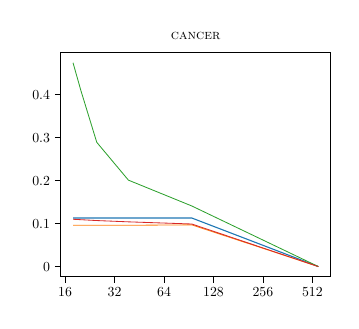
\begin{tikzpicture}[
scale=0.5
]

\definecolor{crimson2143940}{RGB}{214,39,40}
\definecolor{darkgray176}{RGB}{176,176,176}
\definecolor{darkorange25512714}{RGB}{255,127,14}
\definecolor{forestgreen4416044}{RGB}{44,160,44}
\definecolor{steelblue31119180}{RGB}{31,119,180}

\begin{axis}[
tick align=outside,
tick pos=left,
title={\sc cancer},
x grid style={darkgray176},
xmin=-8.8, xmax=536.8,
xtick style={color=black},
xtick={-100,0,100,200,300,400,500,600},
xticklabels={0,16,32,64,128,256,512,},
y grid style={darkgray176},
ymin=-0.0237, ymax=0.4977,
ytick style={color=black}
]
\addplot [thick, steelblue31119180]
table {%
16 0.113
32 0.113
64 0.113
128 0.113
256 0.113
512 0
};
\addplot [semithick, darkorange25512714]
table {%
16 0.096
32 0.096
64 0.096
128 0.096
256 0.097
512 0
};
\addplot [semithick, forestgreen4416044]
table {%
16 0.474
32 0.409
64 0.289
128 0.201
256 0.141
512 0
};
\addplot [semithick, crimson2143940]
table {%
16 0.11
32 0.109
64 0.107
128 0.104
256 0.099
512 0
};
\end{axis}

\end{tikzpicture}

  \end{minipage}
  \hfill
  \begin{minipage}[t]{.12\textwidth}
    \raggedleft
    % This file was created with tikzplotlib v0.10.1.
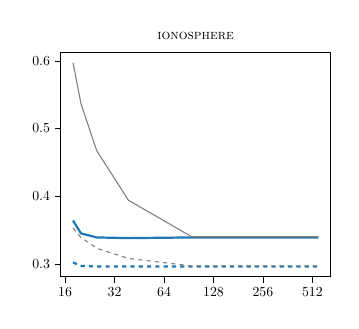
\begin{tikzpicture}[
scale=0.5
]

\definecolor{darkgray176}{RGB}{176,176,176}
\definecolor{gray}{RGB}{128,128,128}
\definecolor{steelblue31119180}{RGB}{31,119,180}

\begin{axis}[
tick align=outside,
tick pos=left,
title={\sc ionosphere},
x grid style={darkgray176},
xmin=-8.8, xmax=536.8,
xtick style={color=black},
xtick={-100,0,100,200,300,400,500,600},
xticklabels={0,16,32,64,128,256,512,},
y grid style={darkgray176},
ymin=0.28095, ymax=0.61205,
ytick style={color=black}
]
\addplot [ultra thick, steelblue31119180]
table {%
16 0.364
32 0.345
64 0.339
128 0.338
256 0.339
512 0.339
};
\addplot [ultra thick, steelblue31119180, dashed]
table {%
16 0.302
32 0.297
64 0.296
128 0.296
256 0.296
512 0.296
};
\addplot [thick, gray]
table {%
16 0.597
32 0.537
64 0.467
128 0.394
256 0.34
512 0.34
};
\addplot [thick, gray, dashed]
table {%
16 0.353
32 0.339
64 0.323
128 0.308
256 0.297
512 0.297
};
\end{axis}

\end{tikzpicture}

  \end{minipage}
  \hfill
  \begin{minipage}[t]{.12\textwidth}
    \raggedleft
    % This file was created by tikzplotlib v0.9.8.
\begin{tikzpicture}[scale=0.5]

\definecolor{color0}{rgb}{0.274509803921569,0.509803921568627,0.705882352941177}
\definecolor{color1}{rgb}{1,0.549019607843137,0}

\begin{axis}[
height=\figureheight,
tick align=outside,
tick pos=left,
title={\sc{Glass}},
width=\figurewidth,
x grid style={white!69.0196078431373!black},
xmin=-5, xmax=105,
xtick style={color=black},
xtick={-20,0,20,40,60,80,100,120},
xticklabels={\ensuremath{-}20,0,20,40,60,80,100,120},
y grid style={white!69.0196078431373!black},
ymin=0.645730930143993, ymax=1.81802513016566,
ytick style={color=black}
]
\path [draw=color0, fill=color0, opacity=0.1]
(axis cs:1,1.49771547138196)
--(axis cs:1,1.18952652316133)
--(axis cs:1,1.18266373930492)
--(axis cs:5,0.96605549198983)
--(axis cs:9,0.857698870422498)
--(axis cs:15,0.78946981593607)
--(axis cs:19,0.809266568098092)
--(axis cs:39,0.762809039558936)
--(axis cs:59,0.699017030144978)
--(axis cs:79,0.729237532733376)
--(axis cs:99,0.720662924824656)
--(axis cs:99,1.04896167752313)
--(axis cs:99,1.04896167752313)
--(axis cs:79,0.995374423453727)
--(axis cs:59,1.0311643117542)
--(axis cs:39,1.02993831156299)
--(axis cs:19,1.03639284358281)
--(axis cs:15,1.04105346761967)
--(axis cs:9,1.02568275842161)
--(axis cs:5,1.16679810278829)
--(axis cs:1,1.35410828283228)
--(axis cs:1,1.49771547138196)
--cycle;

\path [draw=color1, fill=color1, opacity=0.1]
(axis cs:1,1.76473903016467)
--(axis cs:1,1.58753965664686)
--(axis cs:1,1.57139842233233)
--(axis cs:5,1.35246612424739)
--(axis cs:9,1.24713571688454)
--(axis cs:15,1.14321333399575)
--(axis cs:19,1.11838605334277)
--(axis cs:39,0.956363946082652)
--(axis cs:59,0.843593507041992)
--(axis cs:79,0.782856534900766)
--(axis cs:99,0.743711704977892)
--(axis cs:99,1.01490281645003)
--(axis cs:99,1.01490281645003)
--(axis cs:79,1.04688512529527)
--(axis cs:59,1.08499783743299)
--(axis cs:39,1.12512608223656)
--(axis cs:19,1.27061408651308)
--(axis cs:15,1.26826043220348)
--(axis cs:9,1.56711712146726)
--(axis cs:5,1.55216843320769)
--(axis cs:1,1.6887418957198)
--(axis cs:1,1.76473903016467)
--cycle;

\addplot [semithick, color0]
table {%
1 1.34362099727164
1 1.2683860110686
5 1.06642679738906
9 0.941690814422055
15 0.915261641777871
19 0.922829705840453
39 0.896373675560965
59 0.865090670949587
79 0.862305978093552
99 0.884812301173894
};
\addplot [semithick, color1]
table {%
1 1.67613934340577
1 1.63007015902607
5 1.45231727872754
9 1.4071264191759
15 1.20573688309961
19 1.19450006992792
39 1.0407450141596
59 0.96429567223749
79 0.914870830098019
99 0.879307260713959
};
\end{axis}

\end{tikzpicture}

  \end{minipage}
  \hfill
  \begin{minipage}[t]{.12\textwidth}
    \raggedleft
    % This file was created with tikzplotlib v0.10.1.
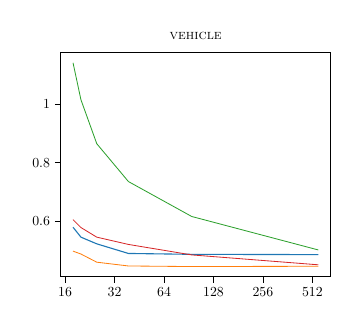
\begin{tikzpicture}[
scale=0.5
]

\definecolor{crimson2143940}{RGB}{214,39,40}
\definecolor{darkgray176}{RGB}{176,176,176}
\definecolor{darkorange25512714}{RGB}{255,127,14}
\definecolor{forestgreen4416044}{RGB}{44,160,44}
\definecolor{steelblue31119180}{RGB}{31,119,180}

\begin{axis}[
tick align=outside,
tick pos=left,
title={\sc vehicle},
x grid style={darkgray176},
xmin=-8.8, xmax=536.8,
xtick style={color=black},
xtick={-100,0,100,200,300,400,500,600},
xticklabels={0,16,32,64,128,256,512,},
y grid style={darkgray176},
ymin=0.408, ymax=1.178,
ytick style={color=black}
]
\addplot [thick, steelblue31119180]
table {%
16 0.578
32 0.544
64 0.521
128 0.488
256 0.485
512 0.484
};
\addplot [semithick, darkorange25512714]
table {%
16 0.496
32 0.486
64 0.458
128 0.445
256 0.443
512 0.444
};
\addplot [semithick, forestgreen4416044]
table {%
16 1.143
32 1.016
64 0.865
128 0.735
256 0.615
512 0.5
};
\addplot [semithick, crimson2143940]
table {%
16 0.604
32 0.577
64 0.544
128 0.519
256 0.483
512 0.449
};
\end{axis}

\end{tikzpicture}

  \end{minipage}
  \hfill
  \begin{minipage}[t]{.12\textwidth}
    \raggedleft
    % This file was created with tikzplotlib v0.10.1.
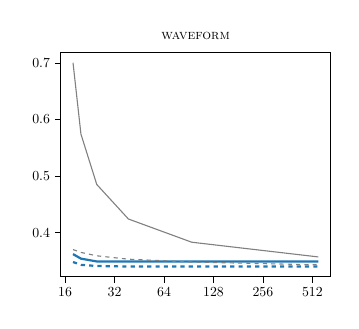
\begin{tikzpicture}[
scale=0.5
]

\definecolor{darkgray176}{RGB}{176,176,176}
\definecolor{gray}{RGB}{128,128,128}
\definecolor{steelblue31119180}{RGB}{31,119,180}

\begin{axis}[
tick align=outside,
tick pos=left,
title={\sc waveform},
x grid style={darkgray176},
xmin=-8.8, xmax=536.8,
xtick style={color=black},
xtick={-100,0,100,200,300,400,500,600},
xticklabels={0,16,32,64,128,256,512,},
y grid style={darkgray176},
ymin=0.322, ymax=0.718,
ytick style={color=black}
]
\addplot [ultra thick, steelblue31119180]
table {%
16 0.362
32 0.354
64 0.349
128 0.349
256 0.349
512 0.349
};
\addplot [ultra thick, steelblue31119180, dashed]
table {%
16 0.348
32 0.343
64 0.341
128 0.34
256 0.34
512 0.34
};
\addplot [thick, gray]
table {%
16 0.7
32 0.574
64 0.485
128 0.424
256 0.383
512 0.357
};
\addplot [thick, gray, dashed]
table {%
16 0.37
32 0.365
64 0.359
128 0.353
256 0.348
512 0.343
};
\end{axis}

\end{tikzpicture}

  \end{minipage}
  \hfill
  \begin{minipage}[t]{.12\textwidth}
    \raggedleft
    % This file was created with tikzplotlib v0.10.1.
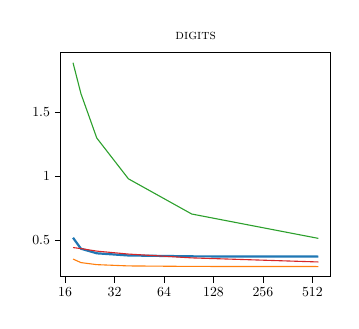
\begin{tikzpicture}[
scale=0.5
]

\definecolor{crimson2143940}{RGB}{214,39,40}
\definecolor{darkgray176}{RGB}{176,176,176}
\definecolor{darkorange25512714}{RGB}{255,127,14}
\definecolor{forestgreen4416044}{RGB}{44,160,44}
\definecolor{steelblue31119180}{RGB}{31,119,180}

\begin{axis}[
tick align=outside,
tick pos=left,
title={\sc digits},
x grid style={darkgray176},
xmin=-8.8, xmax=536.8,
xtick style={color=black},
xtick={-100,0,100,200,300,400,500,600},
xticklabels={0,16,32,64,128,256,512,},
y grid style={darkgray176},
ymin=0.2101, ymax=1.9679,
ytick style={color=black}
]
\addplot [ultra thick, steelblue31119180]
table {%
16 0.516
32 0.43
64 0.394
128 0.377
256 0.37
512 0.368
};
\addplot [thick, darkorange25512714]
table {%
16 0.349
32 0.321
64 0.305
128 0.295
256 0.291
512 0.29
};
\addplot [thick, forestgreen4416044]
table {%
16 1.888
32 1.646
64 1.298
128 0.978
256 0.702
512 0.511
};
\addplot [thick, crimson2143940]
table {%
16 0.439
32 0.431
64 0.411
128 0.388
256 0.358
512 0.326
};
\end{axis}

\end{tikzpicture}

  \end{minipage}
  \hfill
  \begin{minipage}[t]{.12\textwidth}
    \raggedleft
    % This file was created with tikzplotlib v0.10.1.
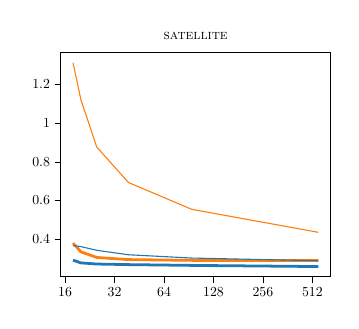
\begin{tikzpicture}[
scale=0.5
]

\definecolor{darkgray176}{RGB}{176,176,176}
\definecolor{darkorange25512714}{RGB}{255,127,14}
\definecolor{steelblue31119180}{RGB}{31,119,180}

\begin{axis}[
tick align=outside,
tick pos=left,
title={\sc satellite},
x grid style={darkgray176},
xmin=-8.8, xmax=536.8,
xtick style={color=black},
xtick={-100,0,100,200,300,400,500,600},
xticklabels={0,16,32,64,128,256,512,},
y grid style={darkgray176},
ymin=0.2053, ymax=1.3647,
ytick style={color=black}
]
\addplot [line width=2pt, darkorange25512714]
table {%
16 0.379
32 0.334
64 0.305
128 0.294
256 0.29
512 0.289
};
\addplot [line width=2pt, steelblue31119180]
table {%
16 0.291
32 0.277
64 0.271
128 0.268
256 0.264
512 0.258
};
\addplot [thick, darkorange25512714]
table {%
16 1.312
32 1.12
64 0.876
128 0.693
256 0.554
512 0.435
};
\addplot [thick, steelblue31119180]
table {%
16 0.367
32 0.361
64 0.342
128 0.319
256 0.302
512 0.288
};
\end{axis}

\end{tikzpicture}

  \end{minipage}\\[-1em]
  %
  % Legend  
  \definecolor{steelblue31119180}{RGB}{31,119,180}
  \definecolor{darkorange25512714}{RGB}{255,127,14}  
  \newcommand{\myline}[1]{\protect\tikz[baseline=-.5ex,line width=1.6pt]\protect\draw[draw=#1](0,0)--(1.2em,0);}
  \caption{Comparison of convergence in terms of number of inducing points $M$ in NLPD (mean over 10 seeds) on UCI classification tasks: \our (thick) vs.\ subsets (\cite{immer2021improving}, thin). Orange lines (\myline{darkorange25512714}) use the GP mean, whereas blue lines (\myline{steelblue31119180}) the NN MAP estimate as mean. Our \our converges fast for all cases.\looseness-1}
  \label{fig:uci}
  %\vspace*{-6pt}
\end{figure*}



\paragraph{Sparsifying the NN GP}
\label{sec:sparse-dual-gp}
%
Sparse Gaussian processes reduce the computational complexity by representing the GP as a low-rank approximation induced by a sparse set of input points (see \cite{quinonero2005unifying} for an early overview). Given that we have computed the dual variables derived from our neural network predictions and a kernel function, we could essentially employ any of these sparsification methods. In this work, we opt for the approach suggested by \citet{titsias2009variational} (also used in the DTC approximation, see \cite{quinonero2005unifying}), which defines the marginal predictive distribution as $q_{\vu}(f_i)  = \int p(f_i  \mid \vu) \, q(\vu) \, \mathrm{d}\vu$. Given that we have $p(f_i \mid \vu)$ determined by our GP prior, the goal is to find a $q(\vu)$. 

As demonstrated in \cite{adam2021dual}, the posterior under this model bears a structure akin to \cref{eq:gp_pred}. The authors of that paper exploit the dual variables for approximate inference, but write them using the natural parameterization, primarily because this form is more suitable for optimization through natural gradients. In order to link the dual variables defined in \cref{eq:dual_param}, we write them in the sparse GP using the dual variables
%
\begin{equation} \textstyle
  \valpha_{\vu}  =  \sum_{i=1}^N  \vkzi \, \hat{\alpha}_{i}
  \quad \text{and} \quad
  \MBeta_{\vu} =  \sum_{i=1}^N \vkzi \,\hat{\beta}_{i} \, \vkzi^{\T} ,    
\label{eq:dual_sparse}
\end{equation}
%
where the sparse dual variables are now a sum over \emph{all data points}, with $\valpha_{\vu} \in \R^{M}$ and $\MBeta_{\vu} \in \R^{M  \times M}$. Using this sparse definition of the dual variables, our sparse GP posterior takes the following form:
\begin{align}\label{eq:dual_sparse_post}
   \myexpect_{q_{\vu}(\vf)}[f_i] &= \vkzs^{\T} \MKzz^{-1} \valpha_{\vu}, \\
   %\quad \text{and} \quad 
   \textrm{Var}_{q_{\vu}(\vf)}[f_i]  &= k_{ii} - \vkzs^\top [\MKzz^{-1} - (\MKzz + \MBeta_{\vu})^{-1} ]\vkzs, \nonumber
\end{align}
where $\MKzz$ and $\vkzs$ are defined similarly to $\MKxx$ and $\vk_{\vx i}$ but over the inducing points $\{\vz_j\}_{i=1}^M$, $\vz \in \R^{D}$, instead of the full data set $\dataset$. The key quantities we need to make predictions from our sparse GP from the converged neural network are $(\hat{\alpha}_i, \hat{\beta}_i)$ (\cref{eq:dual_param_laplace}) and a kernel function $\kappa$ (\cref{eq-laplace-approx-function-space}). Contrasting \cref{eq:dual_sparse_post} and \cref{eq:gp_pred}, we can see that the computational complexity went from $\mathcal{O}(N^3)$ to $\mathcal{O}(M^3)$, with $M \ll N$.  Crucially, given the structure of our probabilistic model, our sparse dual variables \cref{eq:dual_sparse} are a compact representation of the full model projected using the kernel. 

Unlike our approach, \citet{immer2021improving} employ a subset of the data points to construct a sparse GP, reducing computational complexity. However, the method could be considered less principled for building a sparse model, as it ignores contribution from the complete data set. It is important to note that the sparsifying process is independent of the approximate inference technique because the dual variables of \cref{eq:dual_param} are computed using \cref{eq-empirical-risk} and a Laplace approximation. More complicated inference techniques, such as variational inference, could be used, but given its simplicity, in our experiments we used the Laplace-GGN approximation with the trained neural network. Furthermore, our dual variable view of approximate inference means we do not need to retrain a separate sparse GP.\looseness-2
% \todo{shouldn't this sentence be clear from the context? we derive the mean/kernel function that define the process, then we have a sparse GP already}





\section{Experiments}
\label{sec:experiments}
%
%\paragraph{Toy examples} For illustrative purposes, we show our approach on a 1D regression problem (\cref{fig:teaser}) and on the 2D {\sc Banana} classification task (\cref{fig:banana}). In \cref{fig:teaser}, we train an MLP neural network with two hidden layers (64 hidden units each, tanh activation) and pass it through \our. The middle panel shows the \our result on a sparse set of data examples, while the rightmost panel demonstrates fast dual conditioning on new data (from \cref{sec:sequential}). In \cref{fig:banana}, we use an MLP with two hidden layers (64 units, sigmoid) and compare to a HMC sampling result obtained by hamiltorch~\cite{cobb2020scaling}. The HMC result is more expressive, but the results are still similar in terms of quantifying the uncertainty in low-data regions.\looseness-1


%Initially, we explore the capability of our method to capture predictive uncertainty through supervised learning tasks using UCI datasets. Subsequently, we extend our supervised learning experiment to image datasets, demonstrating our method's robustness and adaptability to more complex, high-dimensional data. Next, we investigate the potential of our method in a continual learning context, where we update the neural network representation in response to incoming data without necessitating retraining. Lastly, we delve into the realm of reinforcement learning to ascertain the applicability of our approach in an environment that requires sequential decision-making. Each experiment is designed to illuminate a different facet of our method, thereby exemplifying its broad range of applicability and potential for future utilization.

%
%Our experiments seek to answer the following questions:
%\begin{enumerate}
%  \item \textbf{Predictions:} How do predictions with our sparse function-space approximation compare to weight-space approximations? Does our method's ability to consider the full data set offer benefits over subset function-space methods?
%  % \item Does our method's ability to consider the full data set offer benefits over subset function-space methods?
%  \item \textbf{Function-space updates:} How fast are our function-space updates relative to retraining from scratch? Do they improve predictive performance? Are they as good as retraining from scratch?
%  \item \textbf{Uncertainty:} How good are our uncertainty estimates? Can they be used in downstream settings like RL?
%  \item \textbf{Representation:} Is our sparse function-space representation useful for continual learning?
%\end{enumerate}

%
We evaluate \our on eight UCI benchmarks~\cite{UCI}, a variety of binary and multi-class classification tasks with different data set sizes.
We train a two-layer MLP for each of the classification tasks and follow the experiment set up in \cite{immer2021improving}.
%by using the same hyperparameters, performing a hyperparameter search over the prior precision $\delta$,
% We follow \cite{immer2021improving} by using the same hyperparameters, performing a hyperparameter search over the prior precision $\delta$,
% and run the experiment over $10$ random splits.
% That is, after training we construct the \our dual and use the resulting model for uncertainty quantification.
% for the neural network training as in the UCI experiments of
\cref{tbl:uci} (left) shows that \our with $M=256$ either matches or outperforms the predictive performance of the NN MAP, mean-field VI, Bayesian NN, and GLM
predictions %in terms of negative log-predictive density (NLPD).
(baselines from \cite{immer2021improving}).
That is, we match predictive performance despite being sparse.
%
In \cref{tbl:uci} (right) we compare to the subset GP method from \cite{immer2021improving} whilst using only $M=32$ inducing points.
It shows that \our is able to summarize the full data set more effectively than the GP subset method as it maintains predictive performance
whilst using fewer inducing points.
\cref{fig:uci} further shows that as the number of inducing points is lowered $M=512,\ldots, 16$, \our is able to maintain a much better NLPD than the GP subset.
These results demonstrate \our's sparse representation captures information from the entire data set and as a result provides good uncertainty estimates.
We provide further details of our experiments in \cref{app:uci}.
% as well as further results with varying number of inducing poitns ,64,128,256$
% We provide full details of our experiments as well as further experiments with varying number of inducing poitns and further results using $M=16,32,64,128,256$ in \cref{app:uci}.
% benefits of \our in summarizing the full data distribution onto a small set of inducing
% points over just picking a random subset.


\section{Discussion and conclusion}
\label{sec:conclusion}
%
In this paper, we have introduced \our, a novel approach for representing neural networks in sparse function space, exploiting the dual parameters for an efficient low-rank approximation that accommodates information from the entire data distribution. Our method offers a powerful mechanism for capturing predictive uncertainty, updating the model with new data without retraining, and providing a compact representation suitable for continual learning. These aspects were demonstrated in a wide range of problems, data sets, and learning contexts. We showcased our method's ability to capture uncertainty in UCI classification tasks (\cref{sec:uci}), demonstrated robustness on image data sets (\cref{,sec:image}), established its potential for continual learning (\cref{sec:cl-exp}), and finally, verified its applicability in reinforcement learning scenarios (\cref{sec:rl-exp}).

% Discussion points
In practical terms, our model serves a role similar to a sparse GP. However, unlike a conventional GP, it does not provide a straightforward method for specifying or tuning the prior covariance function. This limitation can be addressed indirectly: the architecture of the neural network and the choice of activation functions can be used to implicitly specify and tune the prior assumptions, thereby incorporating a broad range of inductive biases into the model. It is important to note that the Laplace-GGN approach linearizes the network around the MAP solution $\weights^{*}$, resulting in the function-space prior (and consequently the posterior) being only a locally linear approximation of the neural network model.\looseness-1



\clearpage

% In the unusual situation where you want a paper to appear in the
% references without citing it in the main text, use \nocite
% \nocite{langley00}

\bibliography{bibliography}
\bibliographystyle{icml2023}


%%%%%%%%%%%%%%%%%%%%%%%%%%%%%%%%%%%%%%%%%%%%%%%%%%%%%%%%%%%%%%%%%%%%%%%%%%%%%%%
%%%%%%%%%%%%%%%%%%%%%%%%%%%%%%%%%%%%%%%%%%%%%%%%%%%%%%%%%%%%%%%%%%%%%%%%%%%%%%%
% APPENDIX
%%%%%%%%%%%%%%%%%%%%%%%%%%%%%%%%%%%%%%%%%%%%%%%%%%%%%%%%%%%%%%%%%%%%%%%%%%%%%%%
%%%%%%%%%%%%%%%%%%%%%%%%%%%%%%%%%%%%%%%%%%%%%%%%%%%%%%%%%%%%%%%%%%%%%%%%%%%%%%%
\newpage
\appendix
\onecolumn






\end{document}


% This document was modified from the file originally made available by
% Pat Langley and Andrea Danyluk for ICML-2K. This version was created
% by Iain Murray in 2018, and modified by Alexandre Bouchard in
% 2019 and 2021 and by Csaba Szepesvari, Gang Niu and Sivan Sabato in 2022.
% Modified again in 2023 by Sivan Sabato and Jonathan Scarlett.
% Previous contributors include Dan Roy, Lise Getoor and Tobias
% Scheffer, which was slightly modified from the 2010 version by
% Thorsten Joachims & Johannes Fuernkranz, slightly modified from the
% 2009 version by Kiri Wagstaff and Sam Roweis's 2008 version, which is
% slightly modified from Prasad Tadepalli's 2007 version which is a
% lightly changed version of the previous year's version by Andrew
% Moore, which was in turn edited from those of Kristian Kersting and
% Codrina Lauth. Alex Smola contributed to the algorithmic style files.
